

\section{Overlapping Grid Generator: Ogen}


The overlapping grid generation algorithm determines how the different
component grids communicate with each other. The algorithm must also
determine those parts of component grids that are removed from the
computation because that part of the grid either lies underneath 
another grid of higher priority or else that part of the grid lies
outside the domain.

\subsection{Command descriptions} \label{sec:ogen:commands}

\input ogenUpdateInclude.tex

\include changeParametersInclude.tex

\subsection{Algorithm} \label{algorithm}\index{overlapping grid algorithm}

  The algorithm used by Ogen is based upon the original CMPGRD algorithm\cite{CGNS}
with some major changes to improve robustness. The basic improvement is that the new
algorithm initially removes all grid points that lie inside ``holes'' in the grids.
Once the holes have been cut the program can determine explicitly whether there is
enough overlap to generate an overlapping grid and if there is not enough overlap
the offending points can be shown.  


The algorithm for computing the overlapping grid communication is perhaps most
easily understood by reading the following description and also referring to
the series of examples that follow. 

Here are the basic steps in brief:
\begin{description}
  \item[interpolate boundaries:] First try to interpolate points on physical boundaries
      from points on physical boundaries of other grids. 
      \begin{description}
        \item Boundary points that interpolate from the interior of
           other grids are marked either as being 
           an {\tt interiorBoundaryPoint} and an {\tt interpolationPoint} (using a bitwise `or' in the mask).
      \end{description}
  \item[mark hole boundaries:]\index{hole cutting} For each physical boundary find points on other grids that are
      near to and inside or outside of the boundary. After this step the holes in the grid will
      be bounded by a boundary of holes points next to a boundary of interpolation points.
%  \item[discard unused boundary segments:] Parts of some physical boundaries are
%     discarded. At this point the remaining phsyical boundaries form the
%   actual boundary of the domain.
  \item[remove exterior points:] Mark all remaining hole points. These points can be easily swept
       out since the hole cutting algorithm ensures that all holes are bounded by interpolation 
       points. 
%      Remove all points that lie outside of the
%      region enclosed by the remaining physical boundaries. A ray tracing
%      algorithm is used to do this. If a ray starting from a point crosses the
%      boundary an even number of times then the point is outside. Care must
%      be taken when the ray crosses a boundary where two grids overlap as these
%      two crossing must only be counted as one. After this step the topology of
%      the domain has been determined. 
%       The remaining points are guaranteed to lie within the domain.
  \item[classify (improper) interpolation boundary:] \index{interpolation!proper}
        The points on the stairstep boundaries 
     and interpolation boundaries are collected into a list. We first try
     to interpolate these points from other grids using improper interpolation. 
     A point is said to interpolate in an improper way from a grid if it simply lies within
     the grid. Since all the points in the list lie within in the domain they must
     interpolate from some other grid or else there is something wrong. 
     See the section on trouble-shooting for examples when this step fails.
  \item[classify proper interpolation boundary:] \index{interpolation!improper}
        We now take the list of (improperly) interpolated
     points and sort them into one of the following categories:
      \begin{description}
        \item[proper interpolation:] A point of a grid interapolates in a proper way from
          a second grid if the appropriate stencil of points exists on the second grid
          and consists of the correct types of points for the implicit or explicit interpolation.
        \item[discretization point:] An interpolation point on a physical boundary may
            be used as a dicretization point.
      \end{description}
     At the successful completion of this step we should have a valid overlapping grid. 
     There should be no fatal errors in performing the final steps.
  \item[interpolate discretization points:] To reduce the amount of overlap we
        attempt to interpolate discretization points from grids of higher priority.
  \item[remove redundant interpolation points:] \index{interpolation!redundant}
      Any interpolation points that 
      are not needed are removed from the computation. Interpolation points that are
      needed but that can just as well be used as discretization points are turned
      into discretization points.
\end{description}

  

\subsection{Hole cutting algorithm}\index{hole cutting!algorithm}

After checking for interpolation points on boundaries, the next step in the overlapping
grid algorithm is to cut holes. This is the most critical step in the algorithm. 
Each side of a grid that represents a physical boundary is used to cut holes in other grids that
overlay the boundary.

Each face on grid $g$  representing a physical boundary is used to cut holes in other grids.
We also mark points that can interpolate from grid $g$. The goal is to build a barrier of
hole points next to interpolation points that partitions the grid into two regions -- one region
that is inside the domain and one region that is outside the domain.

\begin{itemize}
 \item We check for points, $\xv_g$ on the face of grid $g$ that can interpolate from 
   from another grid $g_2$. These points $\iv_2$ on $g_2$ are potential hole points.
 \item A potential hole point is not cut if it can interpolate from grid $g$, in this case the
     point is marked as an interpolation point.
 \item A potential hole point is NOT cut if the distance to the cutting surface is greater
    than $2 \Delta x_2$ where $\Delta x$ is a measure of the cell size on $g_2$ (currently
  the length of the diagonal of the cell $\iv_2$). Thus in general there will be a layer of
   1-3 points cut near the cutting surface.
 \item A potential hole point is NOT cut if the point $\iv_2$ already can interpolate from another grid $g_3$
    AND the grid $g_3$ shares the same boundary with grid $g$. This condition applies to a thin body and prevents
    points from being cut that are actually inside the domain on the opposite side of the thin body.
\end{itemize}

This section needs to be completed...
\begin{enumerate}
  \item Invert the points $\xv_g$ on grid $g_2$ given coordinates $\rv_{g_2}$.
  \item Compute the {\tt holeMask} mask array which indicates whether a point on the 
    cutting face is inside of outside $g_2$
\begin{verbatim}
 Compute the holeMask:
     holeMask(i1,i2,i3) = 0 : point is outside and not invertible
                        = 1 : point is inside
                        = 2 : point is outside but invertible

                      -------------------------
                      |                       |      
                      |        grid2          |      
    holeMask          |                       |      
      --0---0---2---2---1---1---1---1---1---1---2---2---2---0---0---- cutting curve, grid
                      |                       |      
                      |                       |      
                      |                       |      
                      |                       |      
                      |                       |      
                      -------------------------
\end{verbatim}
  \item The idea now is to mark all points on $g_2$ that are near the cutting face.
\end{enumerate}
  



\subsection{Finding exterior points by ray tracing}

*** Ray tracing is NO longer performed to remove holes points*** but it is used to
generate embedded boundary grids (a future feature).


Exterior points are found by counting the number of times that a semi-infinite ray,
starting from a point $\xv$ and extending in the y-direction to $+\infty$, crosses
the boundaries of the region.  If the ray crosses the boundaries an even number of times then it
is outside the domain.

If a ray crosses the region where two grids overlap then there will appear
to be two points of crossing. We must eliminate one of these points of
crossing or else we will obtain an incorrect result. 

The ray casting algorithm will determine the intersection of the ray with the boundary
surfaces represented as a triangulation of the discrete points.

We keep a list of the positions of intersection, $\xv_i$, as well as the grid and grid
point location of the intersection. Ideally we would only need to check whether two points
of intersection from two different grids are close, $\| \xv_i - \xv_j \| < \epsilon$.
It is not very easy, however, to determine an appropriate value for $\epsilon$. 
If the ray crosses the boundary in a nearly normal direction then the distance $d=\| \xv_i - \xv_j \|$
will be of order the discrepency between the two discrete representations of the surface which
can be estimated by ??

If, however, the ray
crosses the boundary in a nearly tangential direction then the distance $d$
could be as large as the grid spacing in the tangential direction.

There are further complications since the body may represent a very thin surface (such as a wing)
and there may be points of intersection that are close together in physical space 
but actually on opposite sides of the thing body. 

% \end{document}

Thus to perform a robust check we do the following
\begin{enumerate}
  \item Check that two intersecting points belong to two different grids, $g_1 \ne g_2$.
  \item Check that the boundaries on the two grids are shared sides (meaning they 
     belong to the same surface as specified in the grid generation by setting the
     {\tt share} flag).
  \item Check that the grid cells that contain the points of intersection 
     have some vertices that are interpolation points (so that we know we are in a region of overlap) ???
  \item check that the normals to the boundary at the points of intersection 
        point in the same basic direction, $\nv_1\cdot \nv_2 > 0$.
  \item check that the distance $d=\| \xv_i - \xv_j \|$ between the points satsifies
      \begin{align*}
           \alpha &= \vert(\xv_2-\xv_1)\cdot \nv \vert/ \vert\vert (\xv_2-\xv_1) \vert\vert  \qquad 0\le \alpha \le 1\\
           d_n &\equiv \mbox{ normal discrepency} \\
           d_t &\equiv \mbox{ tangential discrepency} \\
           d &\le \alpha d_n + (1-\alpha) d_t  
      \end{align*}
\end{enumerate}

\begin{figure}[hbt]
  \begin{center}
   % \epsfig{file=\figures /ogenRayTrace.share.idraw.ps}
   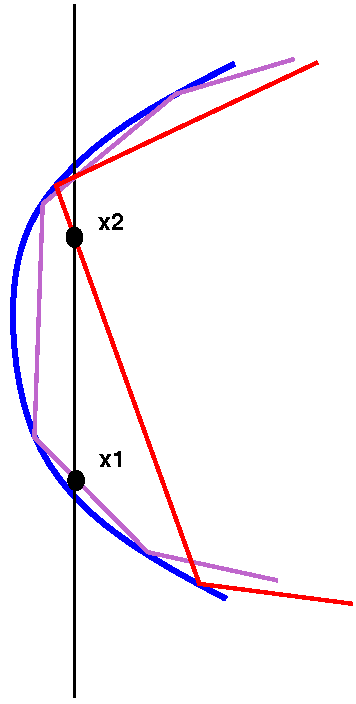
\includegraphics[width=5cm]{\figures/ogenRayTrace_share_idraw}
  \caption{The points of intersection of a ray with a surface covered by two overlapping grids.
      If the ray is nearly tangent to the surface then the two points of intersection may not
      be very close together.}
  \end{center}
\end{figure}

\clearpage
\subsection{Adjusting grid points for the boundary mismatch problem}\index{boundary mismatch}

When the sides of two grids overlap on a boundary then there can be a problem interpolating
one grid from the other if the grids do not match well enough. This problem is especially 
likely if the grids are formed by interpolating data points and the grid spacing is highly 
stretched in the normal direction.

Figure (\ref{mismatch}) shows two grids that share a boundary. If we suppose that the
mapping for the grid is defined by linear interpolation between the grid points then
it is clear that points on the boundary of grid A appear to be well outside or well inside
the boundary of grid B, when actually the boundaries are meant to be the same.

This {\sl boundary mis-match} causes two problems. The first problem, encountered by the grid generator,
is that those boundary points (or even interior points for highly strteched grids)
that appear to be outside the grid should actually be allowed 
to interpolate. The hole cutting algorithm will mark these points as being unusable and outside the grid.
The second problem occurs in PDE solvers. Even if we allow the points to interpolate, the interpolation will
not be very accurate and the solution can look bad.

%% FINISH ME : 
%% \input mismatch.tex

To fix both these problems we adjust the points on grid A so that the boundary points of grid A
are shifted to lie exactly on the boundary of grid B. Other points on grid A are also
shifted, but the amount of the shift decreases the further we are from the boundary.
If the grid is highly stretched then the relative amount we shift the points, compared to the
local grid spacing, decreases as we move away from the boundary. For example if the spacing near
the boundary is $10^{-3}$ compared to the spacing away from the boundary layer then the amount we shift
interior points will be on the order of $10^{-3}$, a very small relative change.
{\bf Note that this shift is only done when we are determining the location of A grid points
in the parameter space of grid B (for interpolation)}. 
The actual grid points are not changed in the {\tt CompositeGrid}
created by the grid generator. Also note that points on grid A may be shifted one amount when interpolating
from grid B, but could be shifted another amount if interpolating from a third grid C.

Referring to figure (\ref{fig:mismatchCorner}) the point $\xv_0$ is shifted to the point $\xv_1$
on the boundary. The point $\xv_2$ is also shifted, but by a smaller amount, that depends
on the distance from the boundary relative to the vector $\wv$ 
\begin{align*}
   \tilde{\xv_2} & \leftarrow \xv_2 + (\xv_1-\xv_0)[ 1 - { (\xv_2-\xv_0)\cdot \wv \over \|\wv\|^2 } ] \\
                 & \equiv     \xv_2 + (\xv_1-\xv_0)[ 1 - { (\xv_2-\xv_0)\cdot \wv \over \|\wv\|^2 } ] \\
                 & \equiv \Sv(\xv_1) \xv_2 
\end{align*}
The {\sl opposite-boundary} vector $\wv$ is chosen to extend from the boundary to the grid points as some
distance from the boundary. We use the grid line that is at least 1/3 of the distance (in index space)
to the opposite side, but at least 10 lines (unless there are fewer than 10 lines). The vector should be
far enough away so that points in the boundary layer are shifted to be inside the other grid, but close enough
so that $\wv$ is nearly parallel to the normal to the boundary.

The shift operator $\Sv$ will project the boundary points of grid A onto the boundary of grid B.

A complication occurs if the more than one side of grid A shares sides with the same grid B, as shown
in figure (\ref{fig:mismatchCorner}). In this case we must determine shifts in multiple directions so that after
these shifts the boundary points on grid A are shifted to lie on the boundary of grid B. We cannot simply 
apply the above algorithm for each side independently.

To fix this problem we sequentially apply the shift operations more than once in order to ensure that
the grids points are projected onto all the shared boundaries. Let $\Sv_0$, $\Sv_1$ and $\Sv_2$
denote the shift mappings in each coordinate direction. In two dimensions, the operator
\[
   \tilde{\xv_2} \leftarrow \Sv_1 \Sv_0 \xv
\]
will not work properly since after the application of $\Sv_1$ the points on boundary 0 can be shifted
off the boundary. However the operator
\[
   \tilde{\xv_2} \leftarrow \Sv_0 \Sv_1 \Sv_0 \xv
\]
would work since the final $\Sv_0$ operator will not change the points on boundary 1 (since the corner
points of grid A have been projected to the corner points of grid B after the two steps $\Sv_1 \Sv_0 \xv$).

Rather than applying $\Sv_0$ twice it is more efficient to define new operators to perform the projection
in only two steps:
\[
   \tilde{\xv_2} \leftarrow \widetilde{\Sv}_1 \widetilde{\Sv}_0 \xv 
\]
We can do this 
\begin{align*}
    \widetilde{\Sv}_0 & =   \Sv_0(\xv_1+\yv) \\
                 \yv  &= \Sv_0(\xv_1)\xv_1 \\
    \widetilde{\Sv}_1 & =   \Sv_1 
\end{align*}

In three-dimensions if we have three adjacent shared faces then 
\begin{align*}
   \tilde{\xv_2} & \leftarrow \widetilde{\Sv}_2 \widetilde{\Sv}_1 \widetilde{\Sv}_0 \xv \\\
    \widetilde{\Sv}_0 & =   \Sv_0 \Sv_2 \Sv_1 \Sv_0 \\
    \widetilde{\Sv}_1 & =   \Sv_1    \\
    \widetilde{\Sv}_1 & =   \Sv_2 
\end{align*}


% However this complication can be fixed using the ideas from trans-finite interpolation. Given 
% shift vectors, $\sv_0(r_0)$, $\sv_1(r_0)$, $\sv_2(r_1)$ and $\sv_3(r_1)$ which define the amount we
% should shift the boundary points on grid A on four sides (in 3D we could have up to 6 sides)
% we can define a composite shift vector of the form
% \begin{align*}
%     \sv(r_0,r_1) = &\phi_0(r_0,r_1) \sv_0(r_0) + \phi_1(r_0,r_1) \sv_1(r_0) \\
%                  + &\phi_2(r_0,r_1) \sv_2(r_1) + \phi_3(r_0,r_1) \sv_3(r_1) \\
%            -\Big\{ &\phi_2(r_0,r_1)\big[\phi_0(r_0,r_1)\sv_0(0) + \phi_1(r_0,r_1) \sv_1(0) \big]  \\
%                   +&\phi_3(r_0,r_1)\big[\phi_0(r_0,r_1)\sv_2(1) + \phi_1(r_0,r_1) \sv_1(1) \big] \Big\} 
% \end{align*}
% We assume that the functions $\phi_i$ satisfy
% \begin{align*}
%     \phi_0(r_0,0)=1, &\quad \phi_0(r_0,1)=0 \\
%     \phi_1(r_0,0)=0, &\quad \phi_1(r_0,1)=1 \\
%     \phi_2(0,r_1)=1, &\quad \phi_2(1,r_1)=0 \\
%     \phi_3(0,r_1)=0, &\quad \phi_3(1,r_1)=1 
% \end{align*}
% and that the shift at the corners match, $\sv_0(0)=\sv_2(0)$, $\sv_0(1)=\sv_3(0)$,
% $\sv_1(0)=\sv_2(1)$, and $\sv_1(1)=\sv_3(1)$. 
% This shift, $\sv(r_0,r_1)$ will perform the correct shift on each side 
% and blend the shifts in the inside. Note the 
% correction term that we must subtract off.


\begin{figure}[hbt]
  \begin{center}
   % 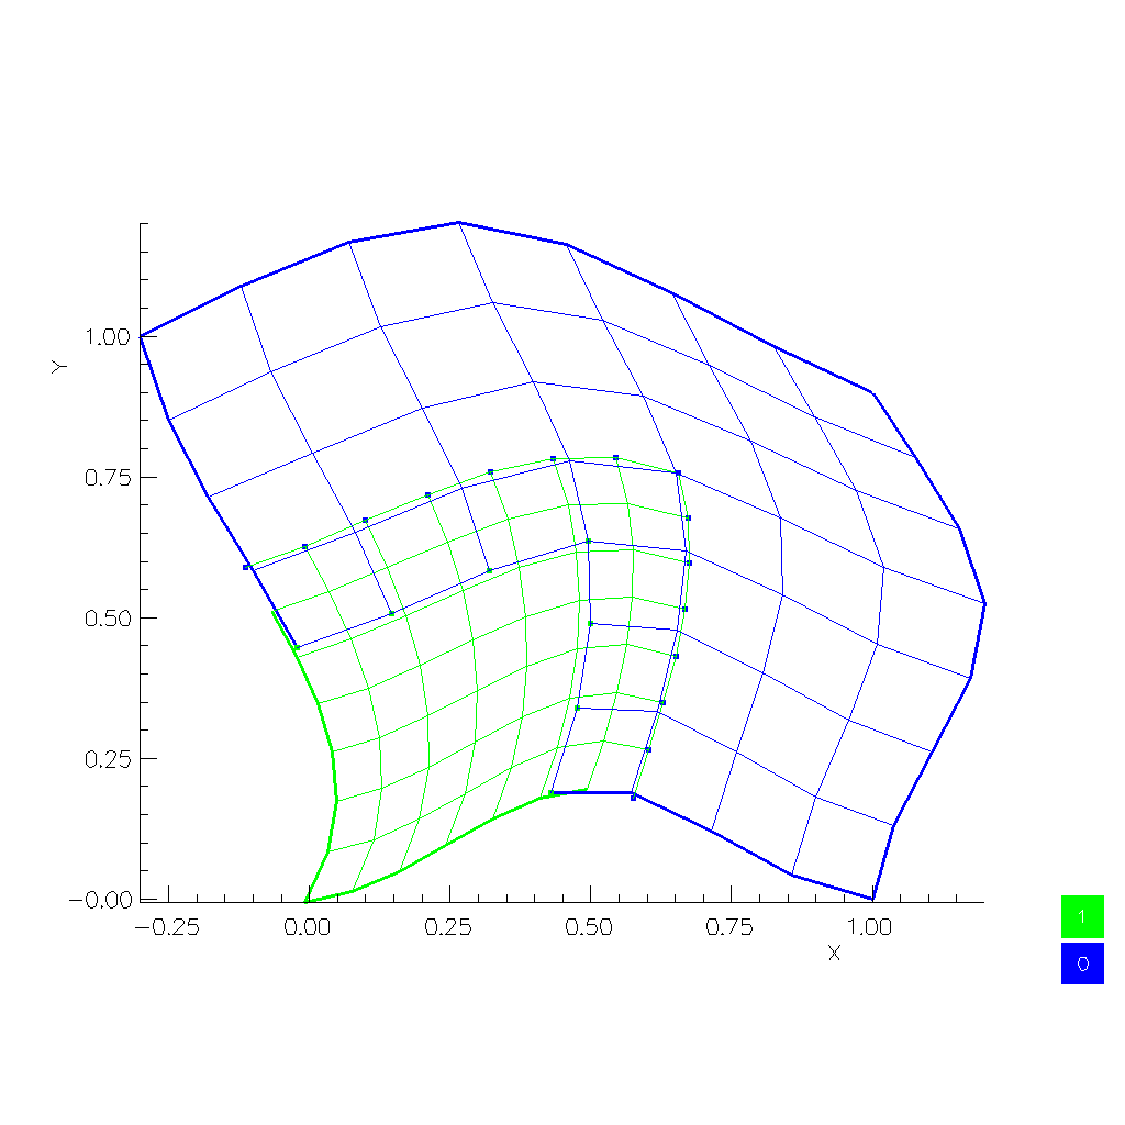
\epsfig{file=\figures/mismatch1.ps,width=3.0in}
   % 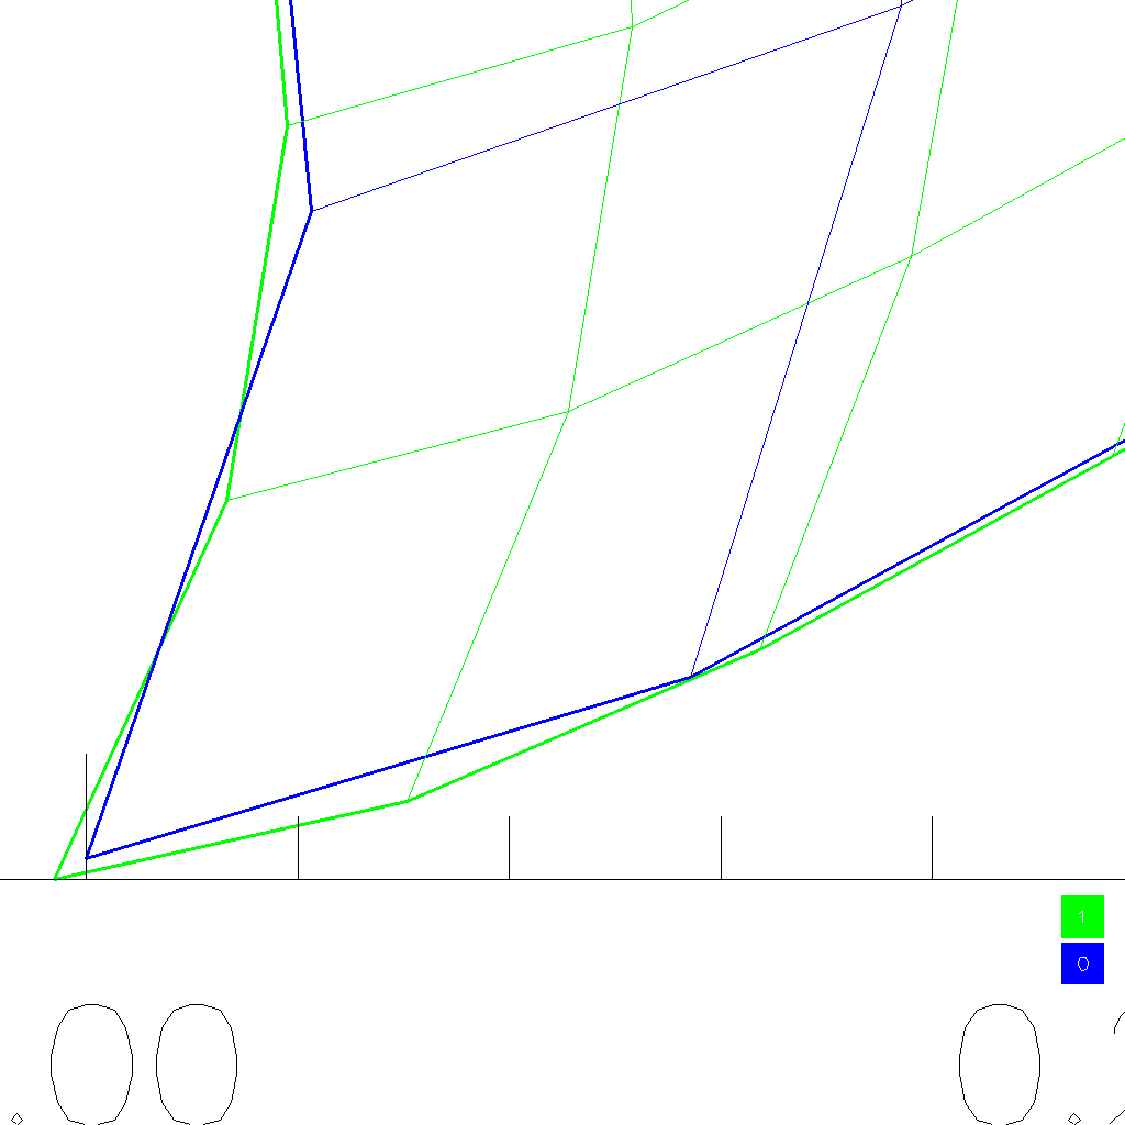
\epsfig{file=\figures/mismatch2.ps,width=3.0in}
   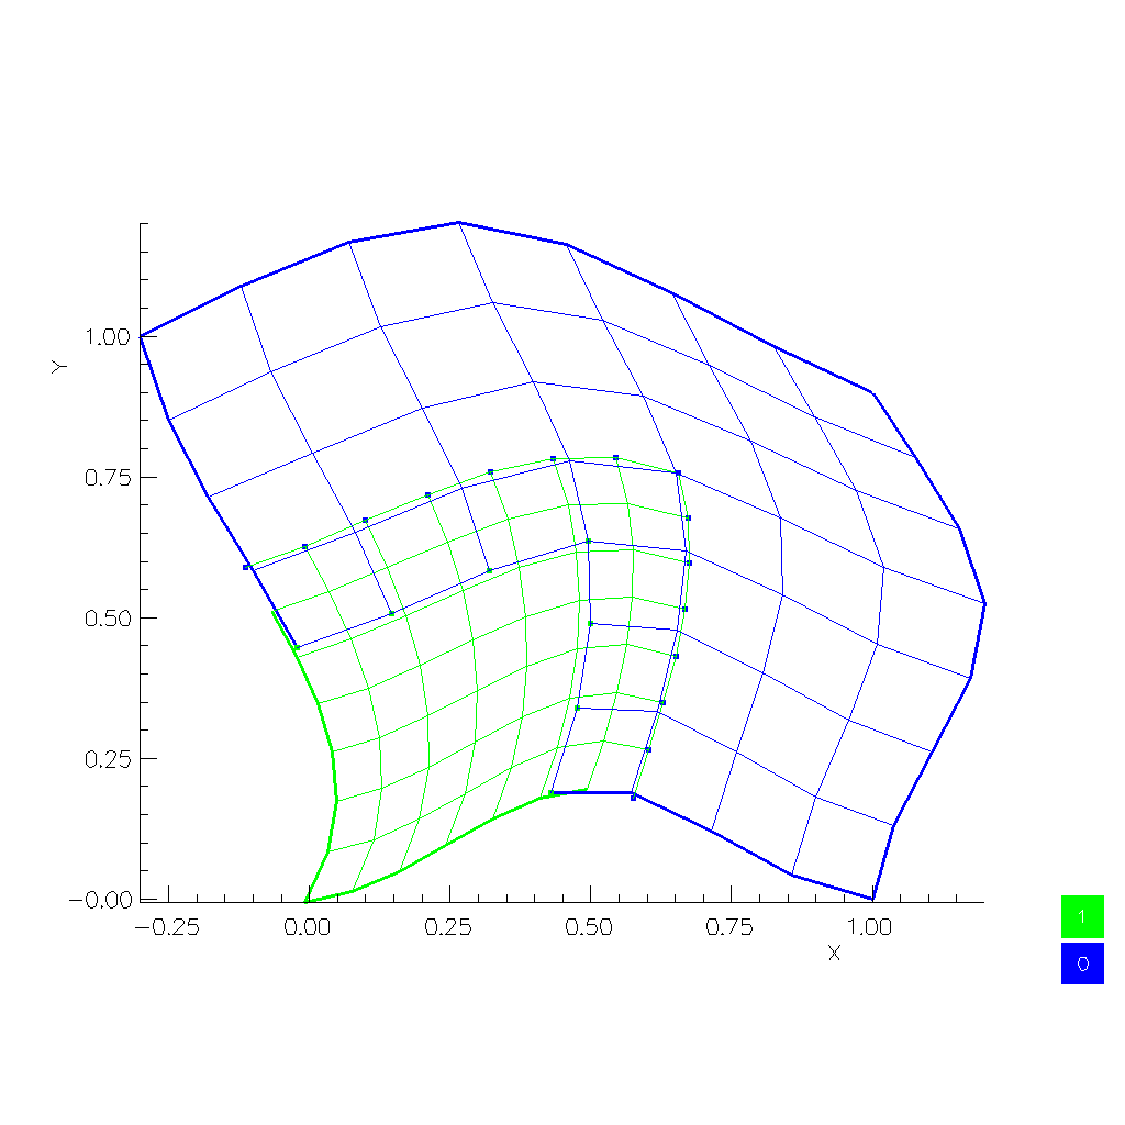
\includegraphics[width=8cm]{\figures/mismatch1}
   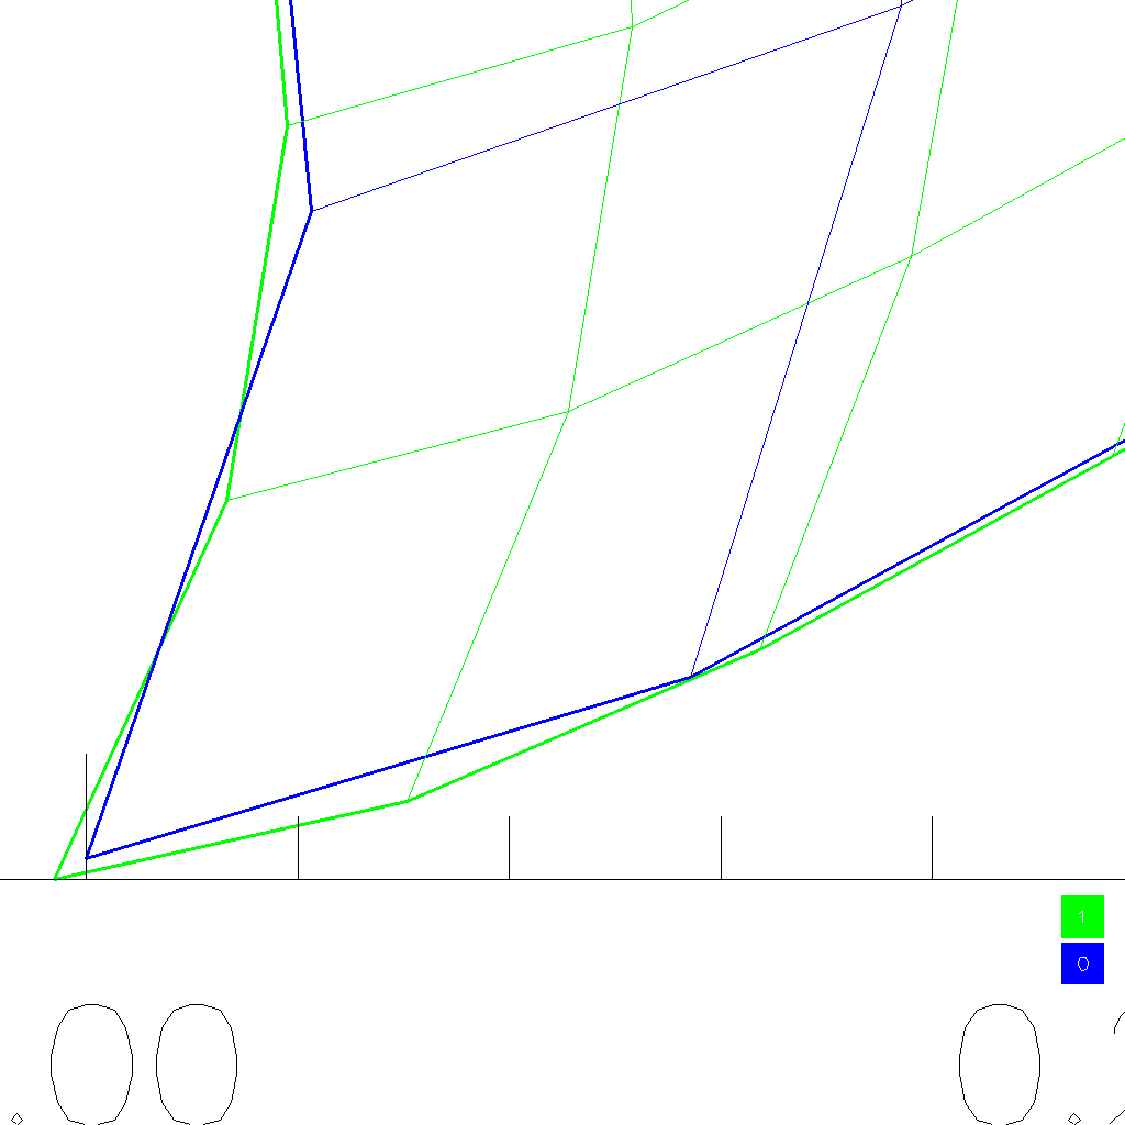
\includegraphics[width=8cm]{\figures/mismatch2}
  \end{center}
  \caption{An overlapping grid testing the mismatch problem, created with {\tt mismatch.cmd}. 
        The refinement grid is artifically translated so that the two boundaries it shares with the base grid do not match.
        The figure on the right is a magnification of the lower left corner, before the overlap algorithm was applied.}
        \label{fig:mismatchCorner}
\end{figure}


\newcommand{\CompositeGrid}{{\tt CompositeGrid}}

\vfill\eject
\subsection{Refinement Grids}\index{refinement grids}

Refinement grids can be added to a {\tt GridCollection} or to a
\CompositeGrid.  The component grids that exist in the original
\CompositeGrid are known as {\bf base grids}.  These grids represent
{\bf refinement level 0}. Refinement grids are added on a particular
base grid and belong to a particular level. Normally the refinement
levels are {\bf properly nested} so that all grids on refinement level
$l$ are contained in the grids on refinement level $l-1$.

A given refinement grid will have only one parent grid on refinement
level 0, i.e. it will belong to only one base grid. A refinement grid
on level $l$ may have more than one parent grid on level $l-1$.

Normally a refinement grid will interpolate its ghost values from
other refinement grids on the same level or from its parent
grids. Points on the parent grid that lie underneath the refinement
will interpolate from the refinement (also known as the child grid).


If refinement grids lie in a region where two base grids overlap, it
is necessary to determine how the refinements interpolate from the
grids they overlap that belong to a different base grid. 

The {\tt updateRefinements} function determines how refinement grids
interpolate from other grids that they overlap. This function does not
determine how a refinement grid interpolates from the grid it has
refined.

If a refinement...

\vfill\eject
\subsection{Improved Quality Interpolation}\index{interpolation!improved quality}

**This is new*** Version 16 or higher.

Normally one wants to avoid having a fine grid interpolate from a coarse
grid or vice versa. Often this can be accomplished through the normal
specification of a priority for each grid. Sometimes, however, using
a single priority per grid is not sufficient.

\begin{figure}[hbt]
  \begin{center}
   % \epsfig{file=\figures /twoCirclesUnimproved.ps,width=.4\linewidth}
   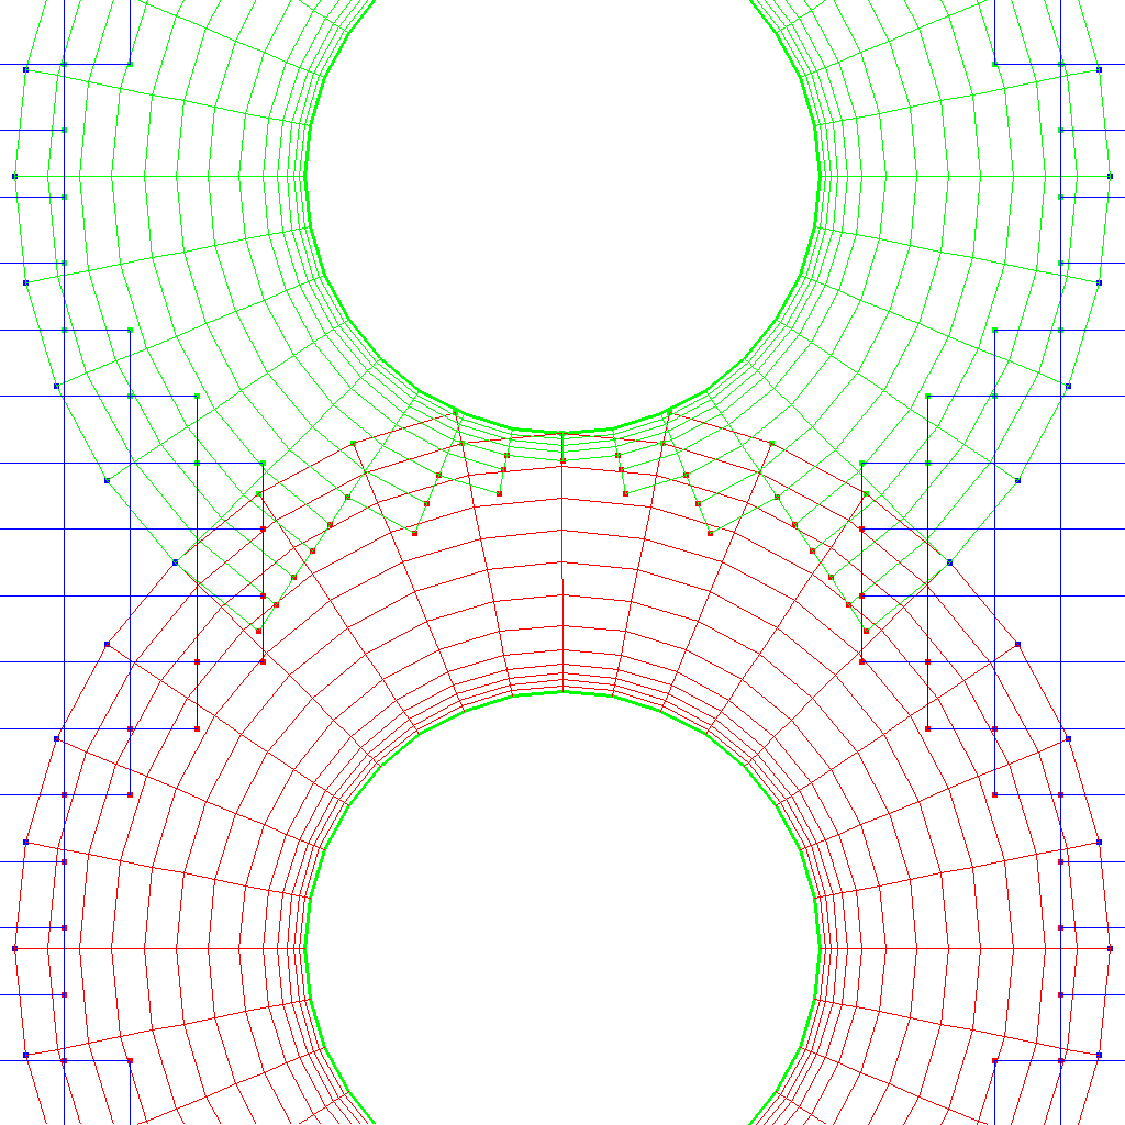
\includegraphics[width=10cm]{\figures/twoCirclesUnimproved}
  \caption{The lower annulus (the highest priority grid ) has points that interpolate from the 
           fine boundary layer grid of the upper annulus. This interpolation will be inaccurate
           if the solution varies rapidly in the boundary layer, and the lower annulus will be unable
           to represent the boundary layer solution accurately. This problem cannot be fixed
           by simply changing the priorities of the grids.  } \label{fig:twoCirclesUnimproved}
  \end{center}
\end{figure}
\begin{figure}[hbt]
  \begin{center}
   % \epsfig{file=\figures /twoCirclesImproved.ps,width=.4\linewidth}
   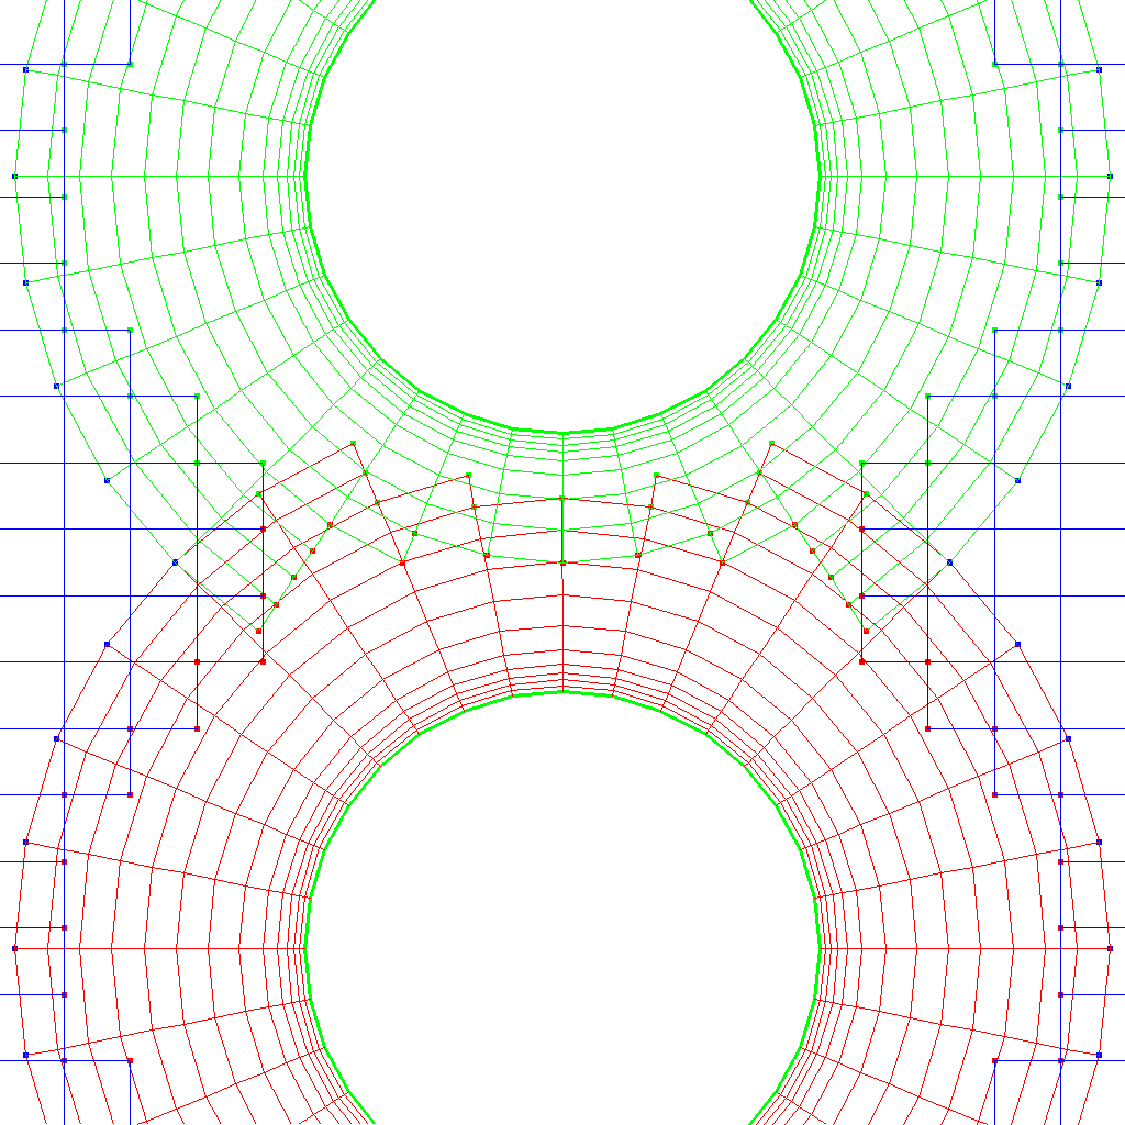
\includegraphics[width=10cm]{\figures/twoCirclesImproved}
  \caption{With the `improved quality' option turned on, the lower annulus no longer interpolates
       from the fine boundary layer of the upper annulus. } \label{fig:twoCirclesImproved}
  \end{center}
\end{figure}

Figure (\ref{fig:twoCirclesUnimproved}) shows a grid where the highest
priority grid (the bottom annulus) interpolates from the fine boundary
layer grid of the top annulus. By turning on the flag to improve the
quality of interpolation the grid shown in figure (\ref{fig:twoCirclesImproved})
results. 


We use a simple measure of the quality of the interpolation to be the relative size of the
grid cells on the two grids involved. 
\[ 
    \text{quality of interpolation} = { \text{cell size of the interpolation point} \over
                                        \text{cell size of the interpolee point} }
\]
The quality is bad (i.e. large) if the interpolee grid cells are smaller.
This simple measure seems adequate for our purposes of preventing coarse grid points
on higher priority grids from interpolating from lower priority grids.


The {\bf algorithm} for removing poor quality points is
\begin{enumerate}
   \item Follow the standard algorithm until all points have been interpolated but redundant points
      have not yet been removed. 
   \item Try to interpolate all points on the finest grid that can interpolate from a lower priority
    grid. (This is not done in the standard case).
   \item Attempt to remove poor quality points from the {\em boundary} of the interpolation point
     region where a point interpolates from a lower priority grid. A point is removed if it is
     not needed for discretization and the quality measure is greater than a specified value (normally
     around 2).  If a point is removed then also check the new {\em boundary}
     points that are now exposed.
   \item After points have been removed we need to go back and update any other interpolation points
     that can no-longer interpolate (since they required some of the points that were deleted).
\end{enumerate}
The algorithm is supposed to be guaranteed to give a valid grid provided a grid could be made
without the improvement steps.

\subsubsection{Note:}

There is a more sophisticated way to measure the quality of interpolation. ***This measure
is not used currently**.

One way to measure the quality of the interpolation is defined as follows. 
We would like the cell at an interpolation point on grid A to be approximately the
same size, shape and orientation as the cells on the interpolee grid B. The vector
\[
     \dv^A_i = {\partial \xv^A \over \partial r_i} \Delta r^A_i 
\] 
measures the grid cell spacing and orientation of the side of the cell along the axis $r_i$ 
of grid A. This vector corresponds to a vector in the parameter space of grid B given by
\[
   \rv^B_i = \left[ {\partial \rv^B \over \partial \xv} \right] \dv_i^A
\]
The length in grid cells of this vector $\rv^B_i$ is approximately
\[
  \left\| \begin{bmatrix} {1\over\Delta r_1^B} & 0 & 0 \\
                          0 & {1\over\Delta r_2^B} & 0  \\
                          0 & 0 & {1\over\Delta r_3^B}  \end{bmatrix} 
      \rv^B_i \right\|
\]
where we have scaled each element by the appropriate grid spacing.
This length should be near 1 for good quality (since the original vector $\dv^A_i$ has a
length of one grid cell).


Thus to measure the quality of all sides on the original cell we can compute
\[
   p = 
   \left\| \begin{bmatrix} {1\over\Delta r_1^B} & 0 & 0 \\
                          0 & {1\over\Delta r_2^B} & 0  \\
                          0 & 0 & {1\over\Delta r_3^B}  \end{bmatrix} 
   \left[ {\partial \rv^B \over \partial \xv} \right]
   \left[ {\partial \xv^A \over \partial \rv }  \right]
          \begin{bmatrix} {\Delta r_1^A} & 0 & 0 \\
                          0 & {\Delta r_2^A} & 0  \\
                          0 & 0 & {\Delta r_3^A}  \end{bmatrix}  \right\|
\]
The interpolation will be defined to be of high quality if this norm is near 1.
In particular we use the quality measure
\[
    q = {1\over2}( p + {1\over p } )
\]
where we prefer points with a smaller value for q.

\clearpage
\section{Treatment of nearby boundaries and the boundaryDiscretisationWidth} \index{boundaryDiscretisationWidth}

** new with version 18**

Figure (\ref{fig:nearby}) shows the grid generated in the case when two boundaries are
very near to one another. The {\tt boundaryDiscretisationWidth} parameter, which is by default 3,
indicates that any boundary point that is a discretisation point should have two interior
neighbouring points so that a one-sided 3-point scheme could be applied on the boundary.
To ensure this condition is satisfied extra points are allowed that normally would not be valid.
The interpolation points that are outside the domain are ``interpolated'' from the nearest point
on the boundary by pretending that the interpolation point has been moved to the boundary. This 
will only be first order accurate interpolation. 

\begin{figure}[hbt]
\begin{center}
   % 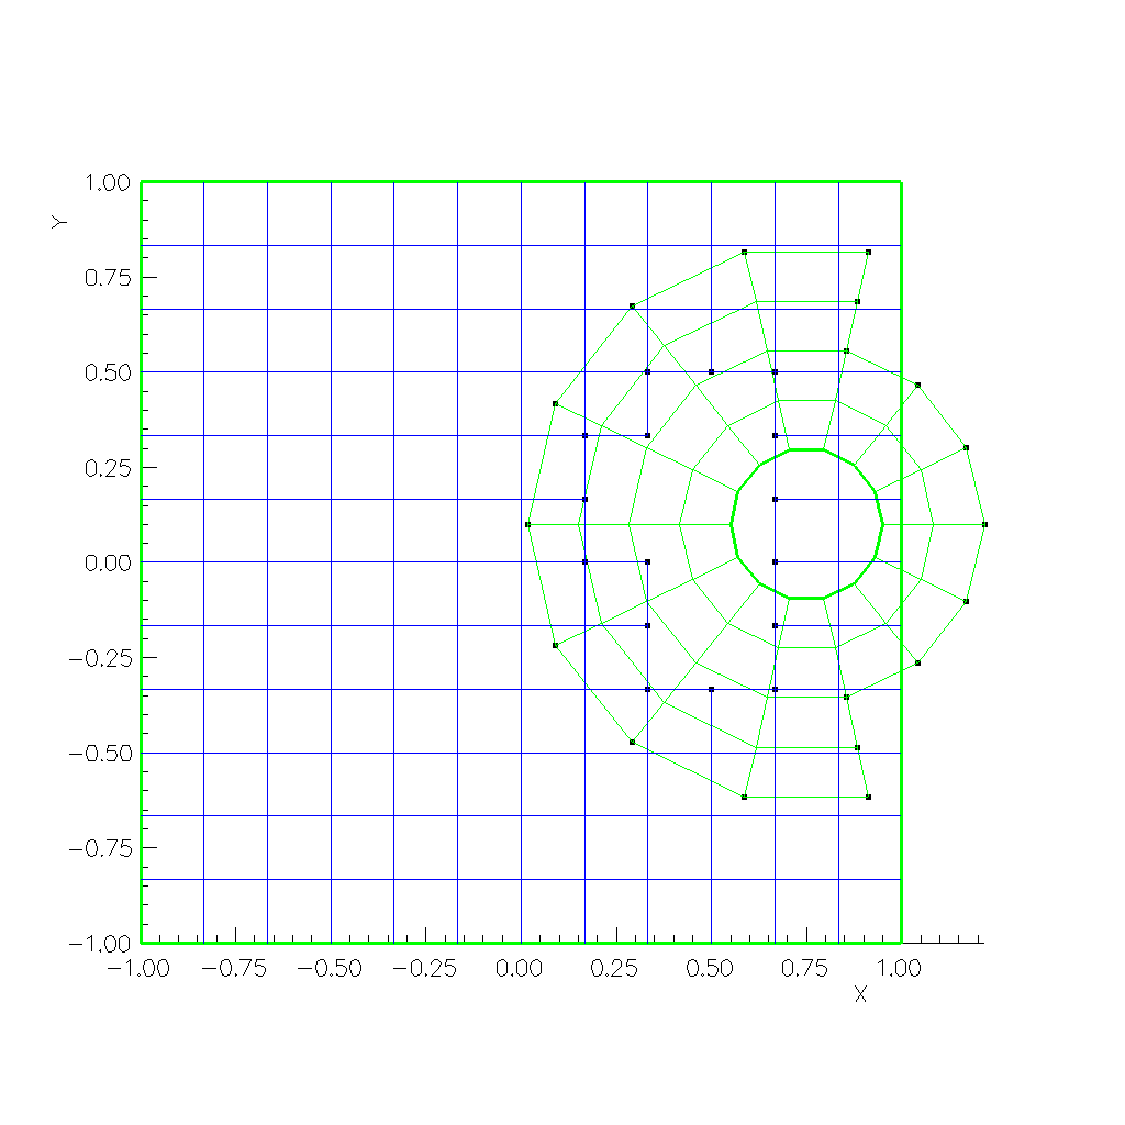
\epsfig{file=\figures/dropNear.ps,height=\figHeight}
   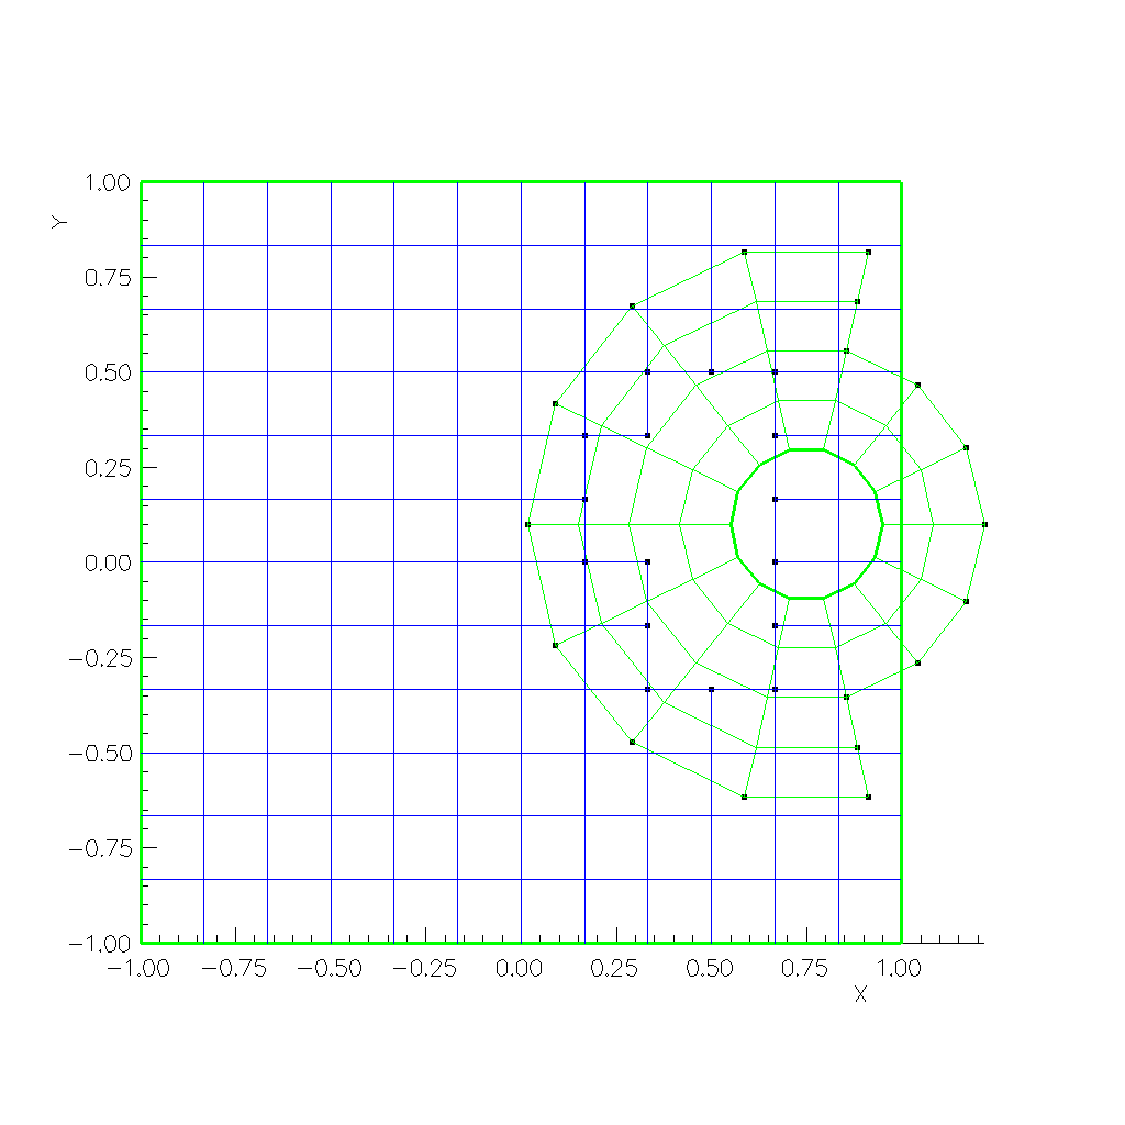
\includegraphics[width=12cm]{\figures/dropNear}
\end{center}
\caption{When two boundaries are nearby to one another the overlapping grid algorithm
   ensures that enough interior grid-points remain next to the boundary points
   to allow the boundary point to be discretised. While not very accurate this approach
   at least allows a grid to be built.} \label{fig:nearby}
\end{figure}

\clearpage
\section{Adaptive Mesh Refinement} \index{adaptive mesh refinement!ogen}

  When refinement grids are added to an overlapping grid and a refinement grid
overlaps an interpolation boundary, the Ogen function {\tt updateRefinement}
should be called. This function will cut holes in the refinement grids and
determine how to interpolate points on the hole-boundary. 

\begin{figure}[hbt]
\begin{center}
   % 
\epsfig{file=cic.refine.grid.eps,width=.75\linewidth}
   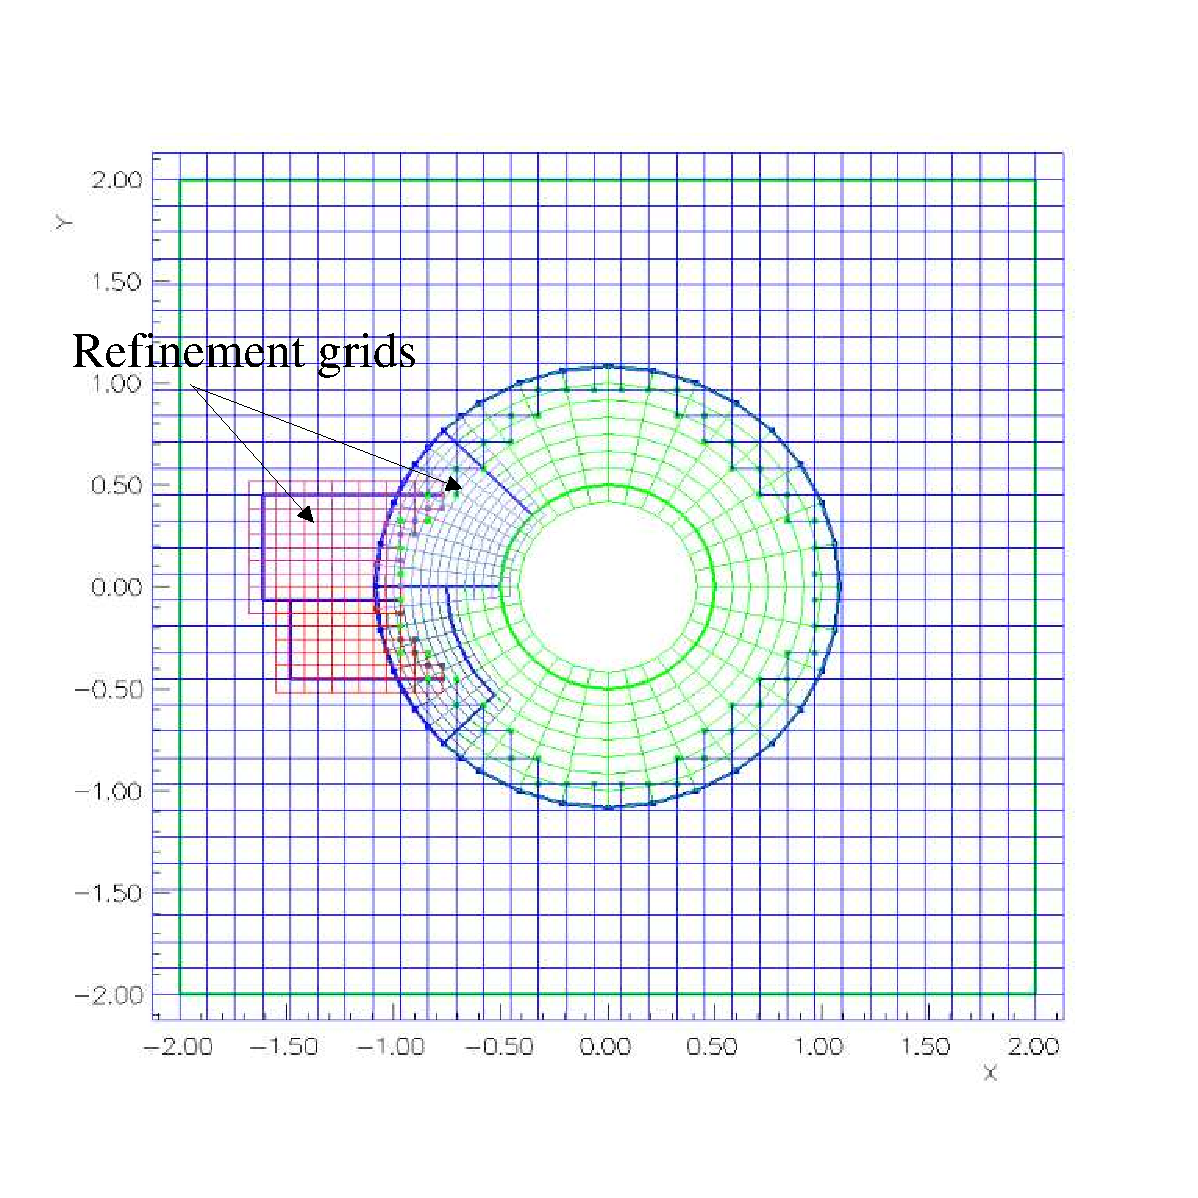
\includegraphics[width=12cm]{\figures/cic_refine_grid}
\end{center}
\caption{When refinement grids are added to an overlapping grid, the {\tt updateRefinement} function
   should be called in order to compute a valid grid.}
\end{figure}

The order of preference for the interpolation of a point on the hole-boundary
of a refinement grid is to
\begin{enumerate}
   \item interpolate from another refinement at the same level and different base grid
   \item interpolate from another refinement at a lower level and different base grid
   \item interpolate from a refinement grid on the same base grid (this case should only be used as a backup
         and should normally not be needed).
\end{enumerate}
  

\subsection{The algorithm for updating refinement meshes added to an overlapping grid.}

  There are two main steps in the algorithm for adding refinement meshes to an overlapping grid.
\begin{enumerate}
  \item Build a mask array for each refinement grid that indicates where holes are and which points
      should be interpolated.
  \item For each interpolation point on the hole boundary, find which grid to interpolate from.
\end{enumerate}
To be efficient, these steps are performed with a different procedure than the normal overlapping
grid algorithm. The mask array is built entirely by looking at the mask array from the base grids.
The interpolation points are determined by looking at the interpolation points on the base grids
in order to determine the likely interpolee grids.





\clearpage
\newcommand{\figWidthc}{10cm}
\subsection{Example: Circle in a Channel}

These figures show the circle in a channel grid at various stages in the overlap algorithm.
\vglue-.1in
  \begin{center}
   % 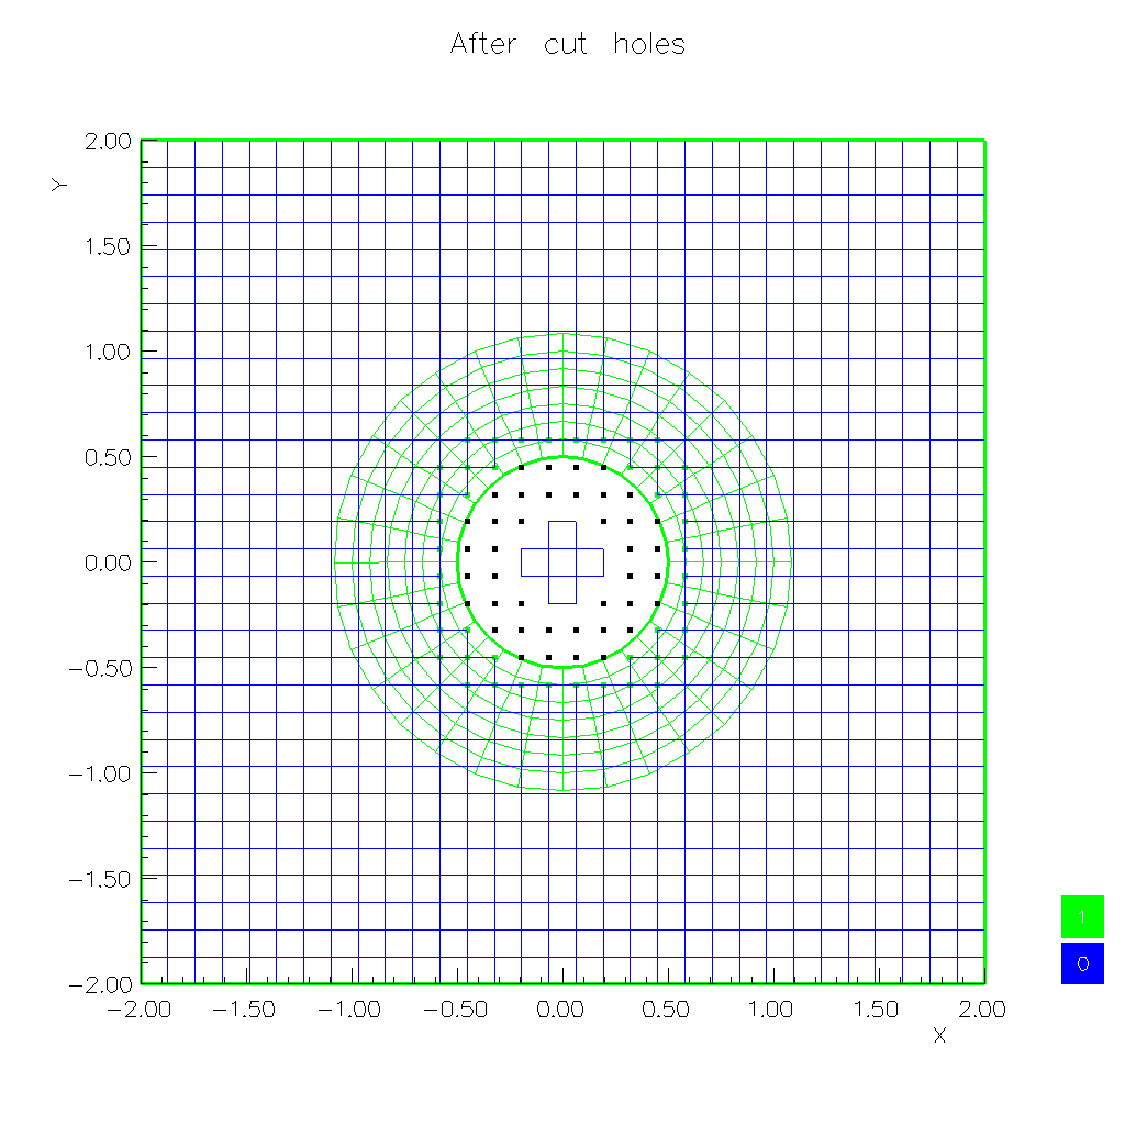
\epsfig{file=\figures/cicCutHoles.ps,height=\figHeight} \\
   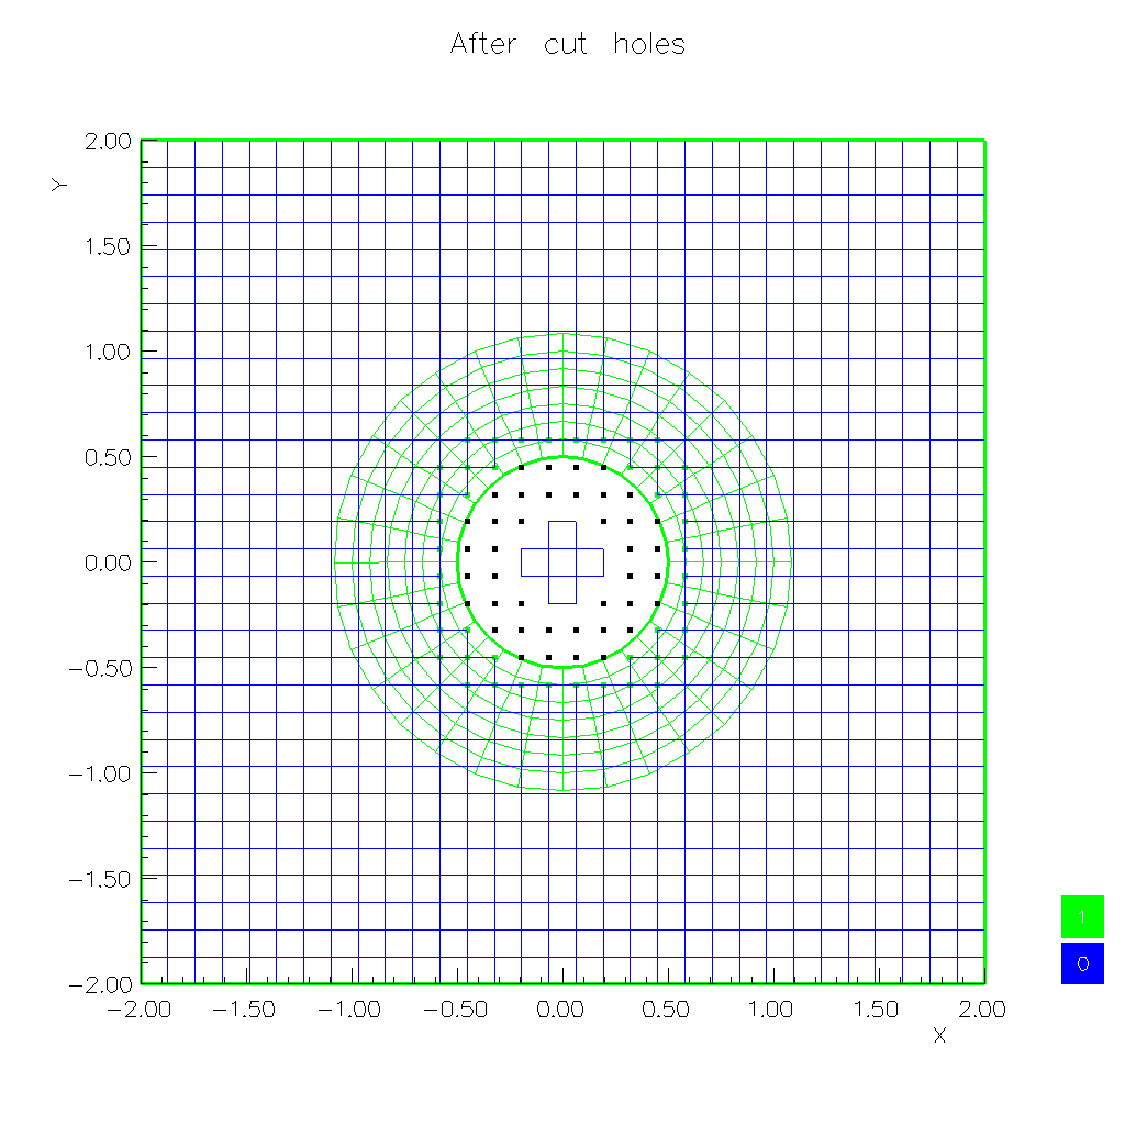
\includegraphics[width=\figWidthc]{\figures/cicCutHoles}\\
  {Grid after cutting holes. Physical boundaries are used to cut
      holes in nearby grids. The hole cutting algorithm will generate a barrier of hole points and
      interpolation points that bounds the entire hole region.}
  \end{center}
\vglue-.5in
  \begin{center}
   % 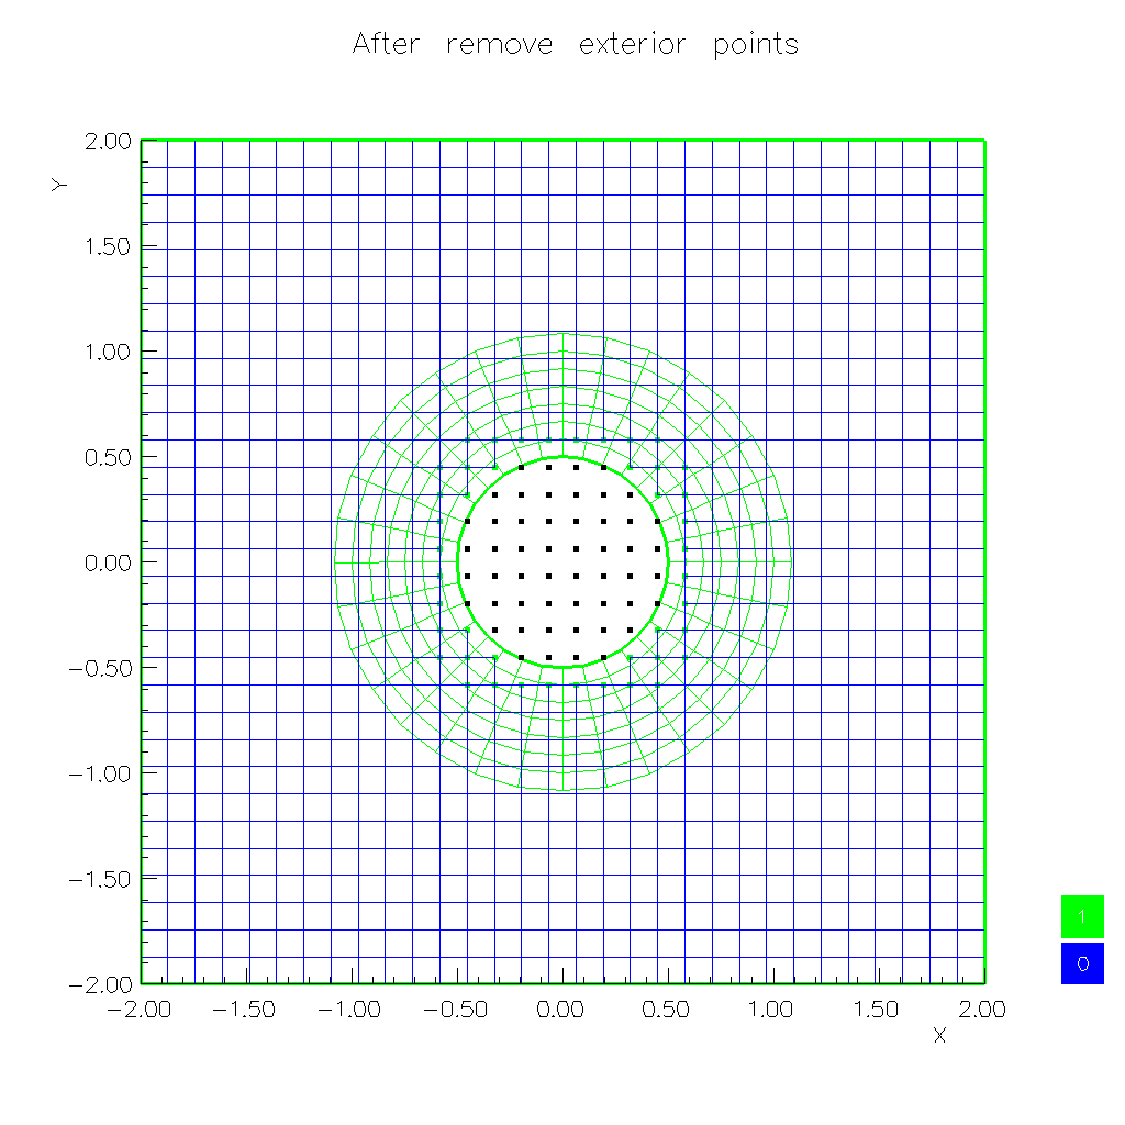
\epsfig{file=\figures/cicRemoveExterior.ps,height=\figHeight} \\
   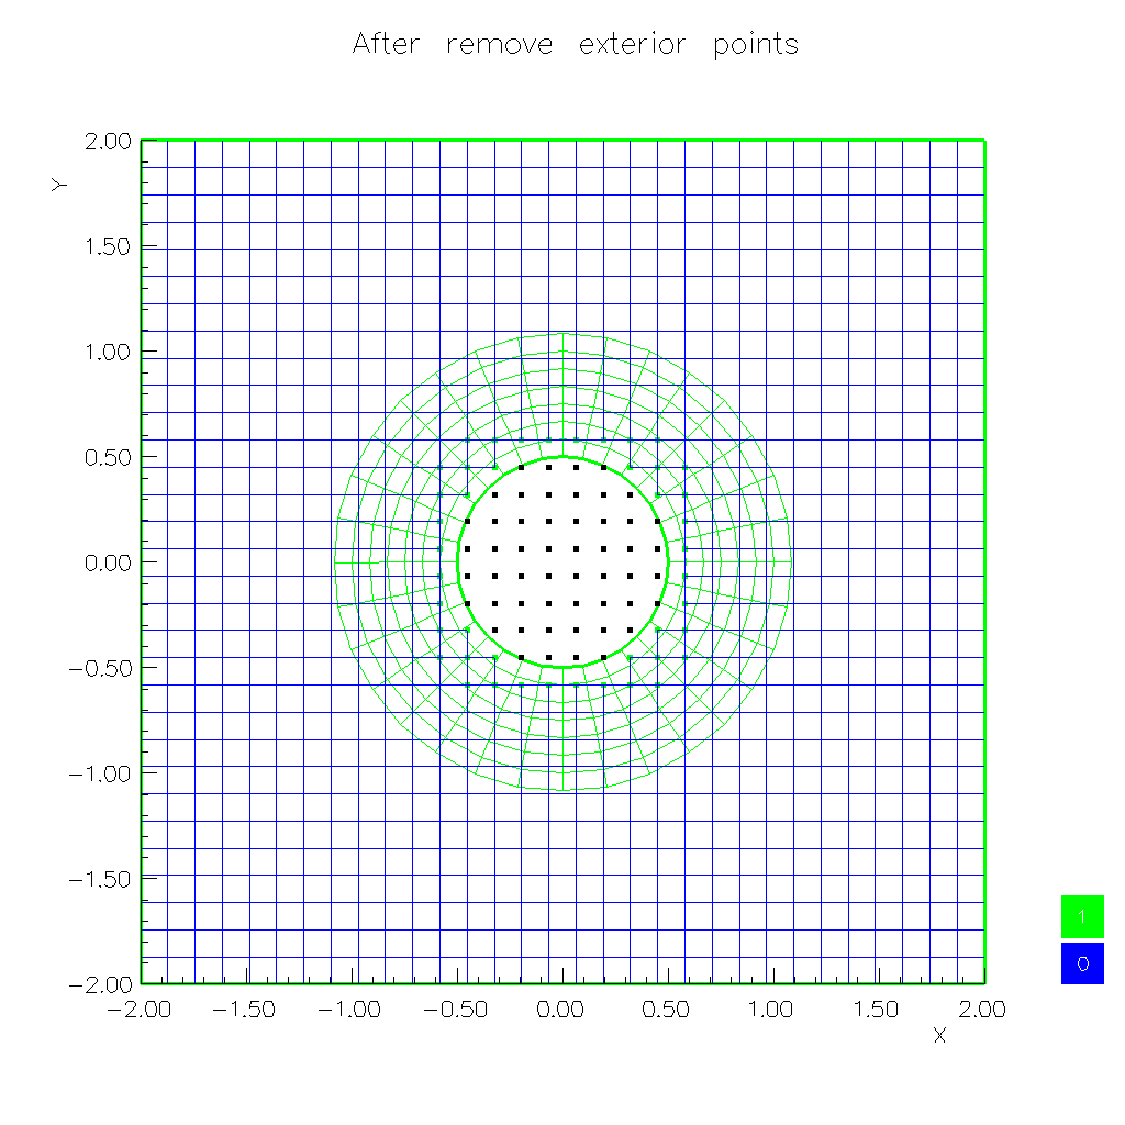
\includegraphics[width=\figWidthc]{\figures/cicRemoveExterior}\\
  {Grid after removing all exterior points. The exterior points are easily swept out
      after the hole boundary has been marked.}
  \end{center}
  \begin{center}
   % 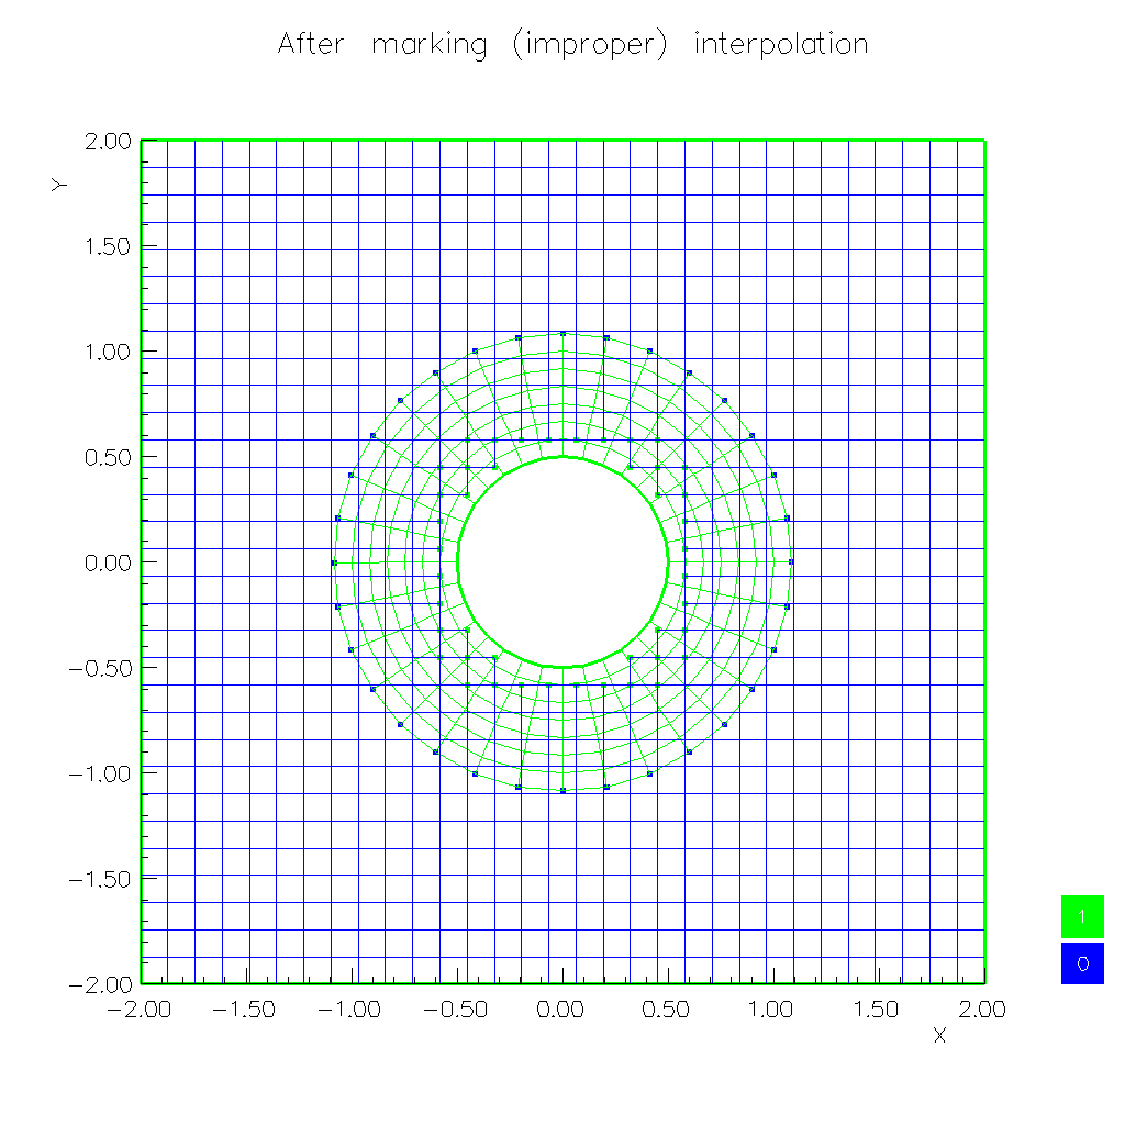
\epsfig{file=\figures/cicImproper.ps,height=\figHeight} \\
   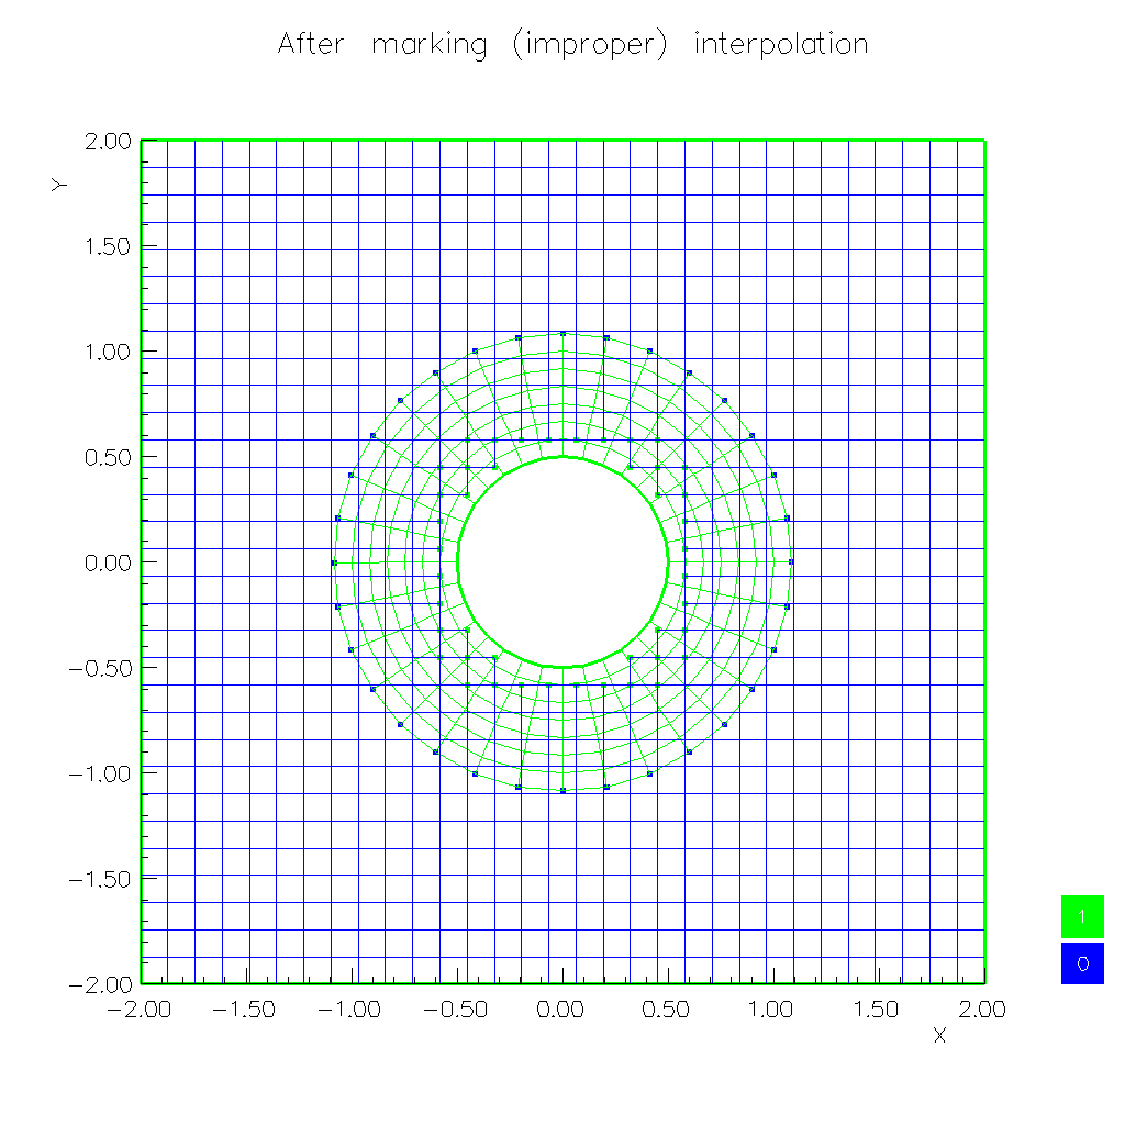
\includegraphics[width=\figWidthc]{\figures/cicImproper}\\
  {Grid after marking (improper) interpolation. These improper interpolation points need only lie
    inside another grid.}
  \end{center}
  \begin{center}
   % 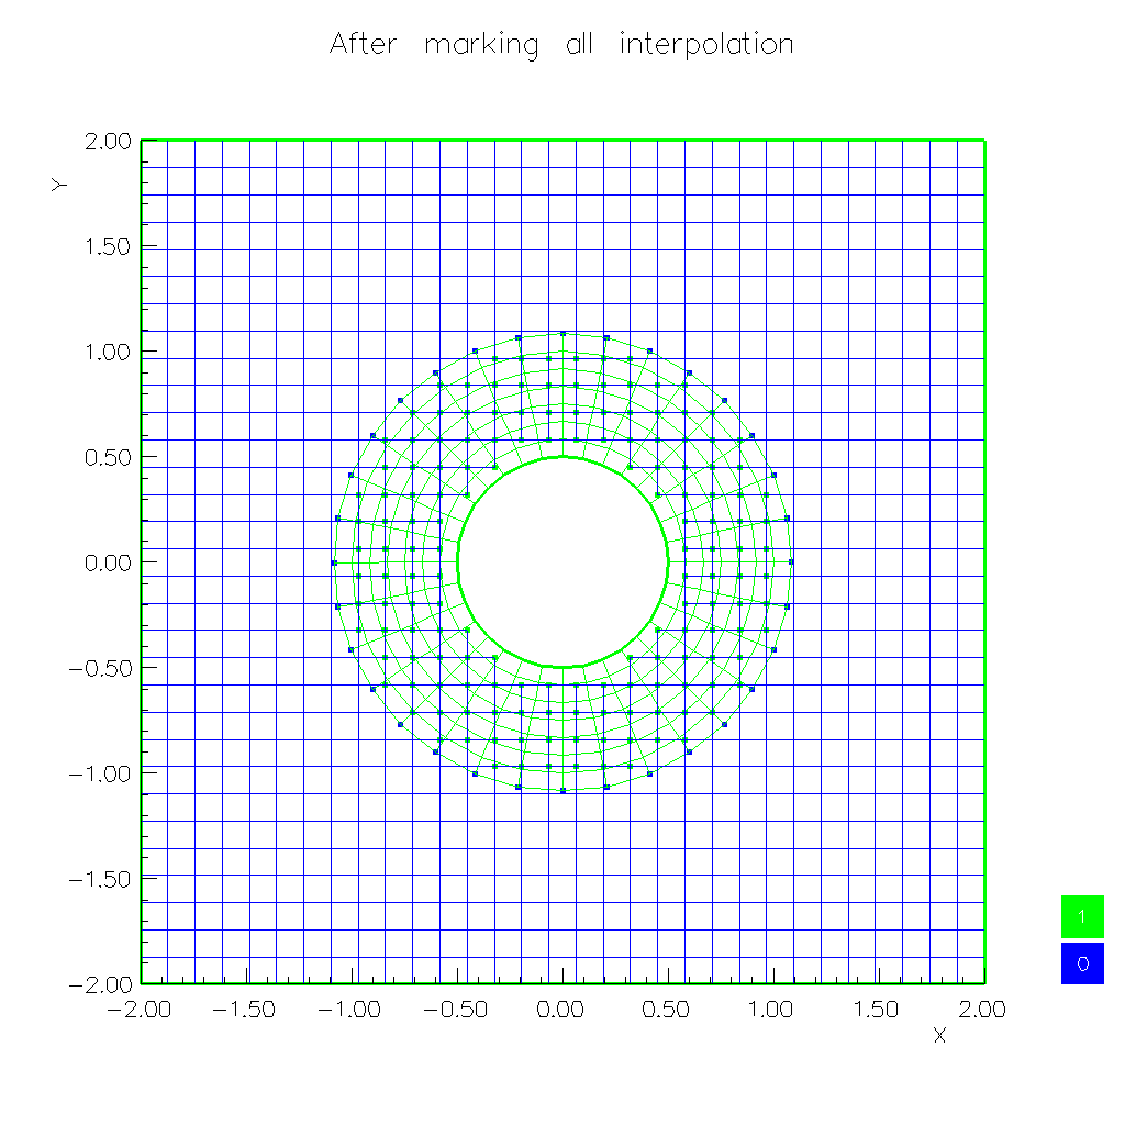
\epsfig{file=\figures/cicAll.ps,height=\figHeight} \\
   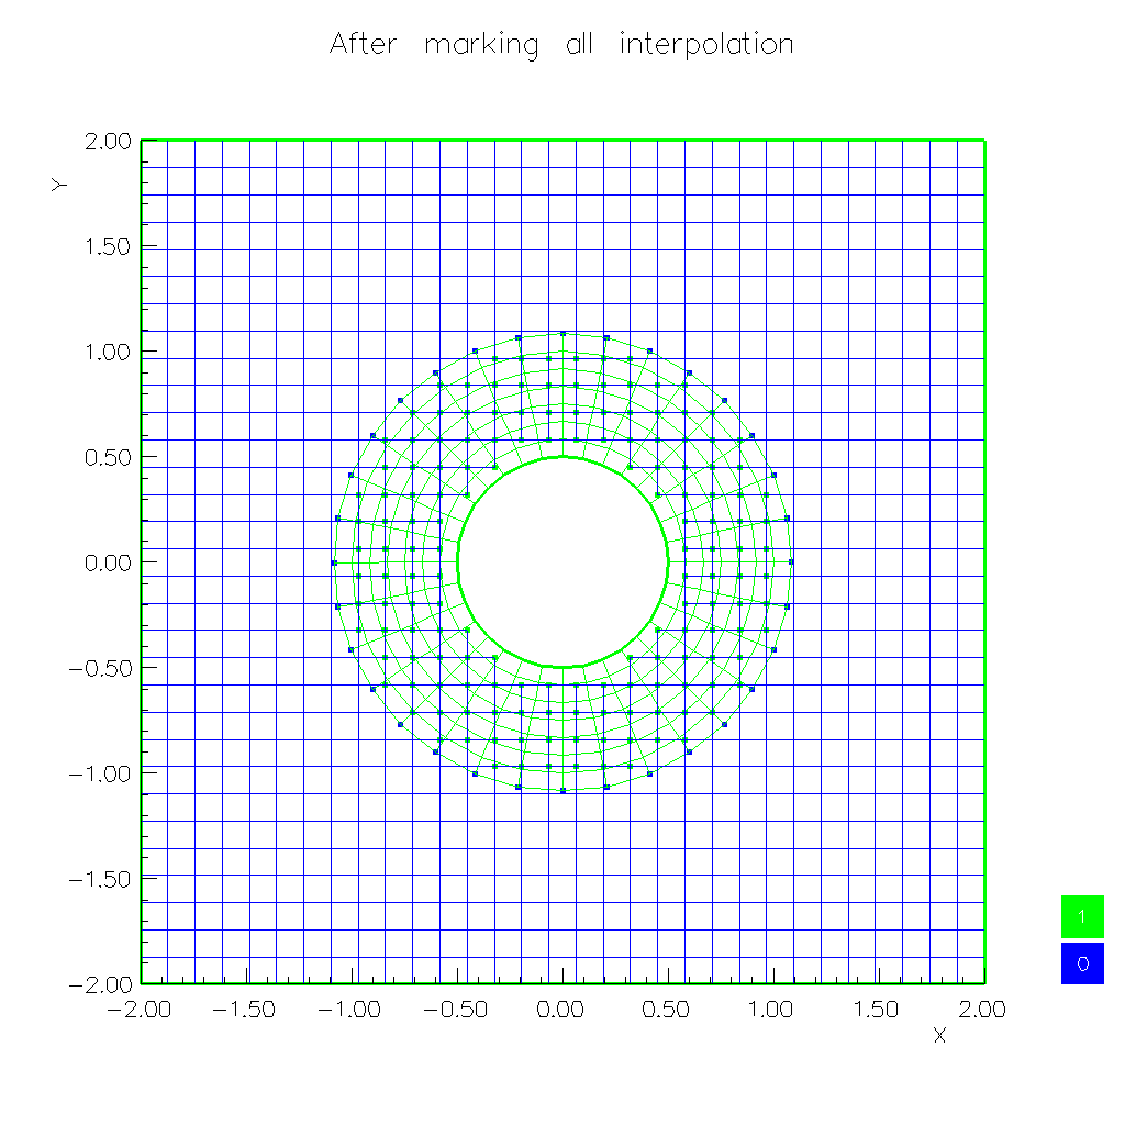
\includegraphics[width=\figWidthc]{\figures/cicAll}\\
  {Grid after marking all (proper) interpolation. We have attempted to interpolate
     discretization points on each grid from grids of higher priority.}
  \end{center}
  \begin{center}
   % 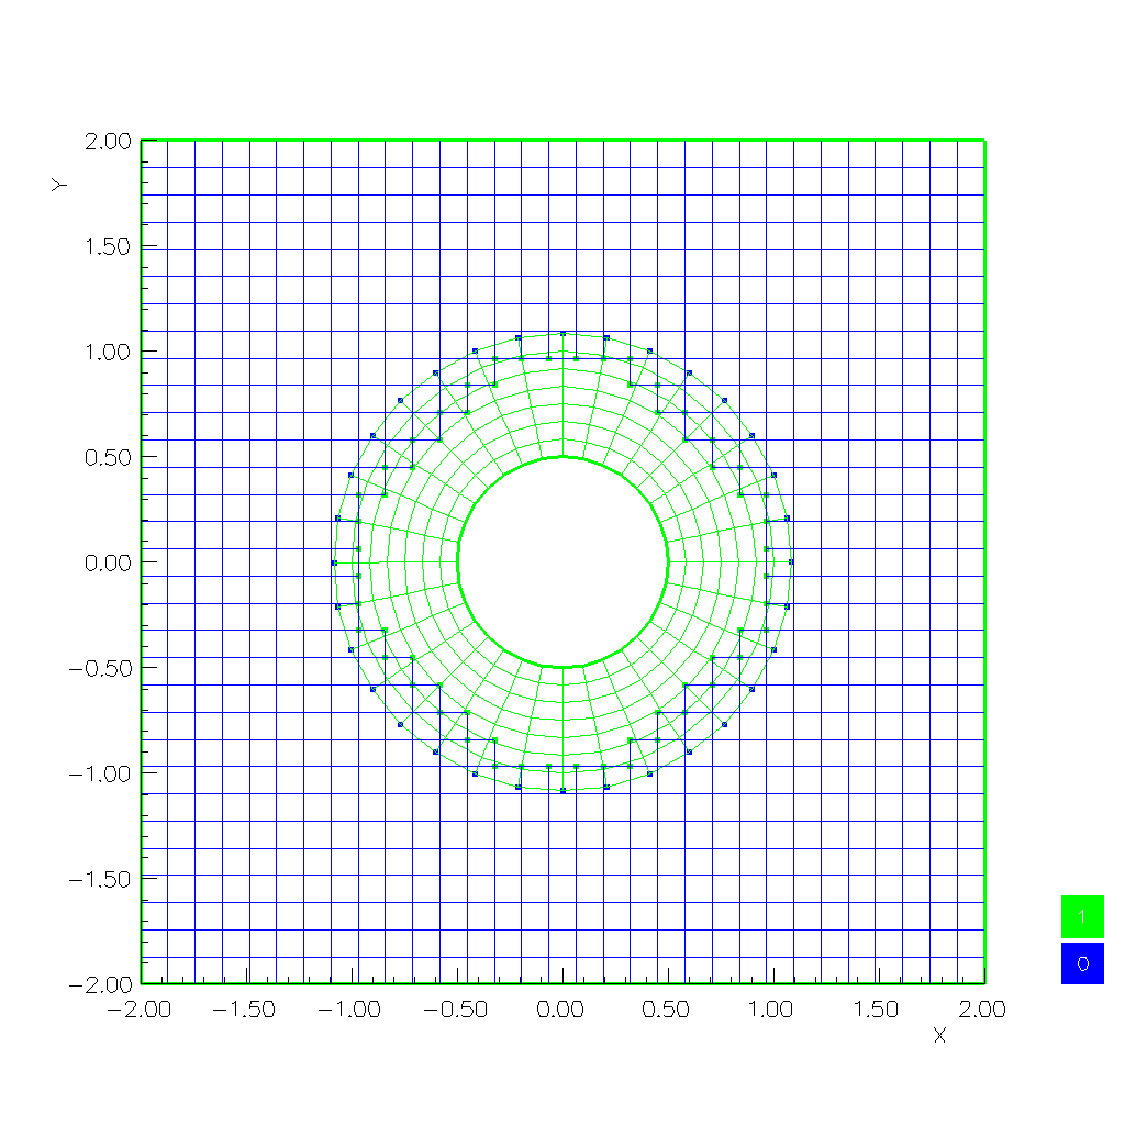
\epsfig{file=\figures/cicDone.ps,height=\figHeight}\\
   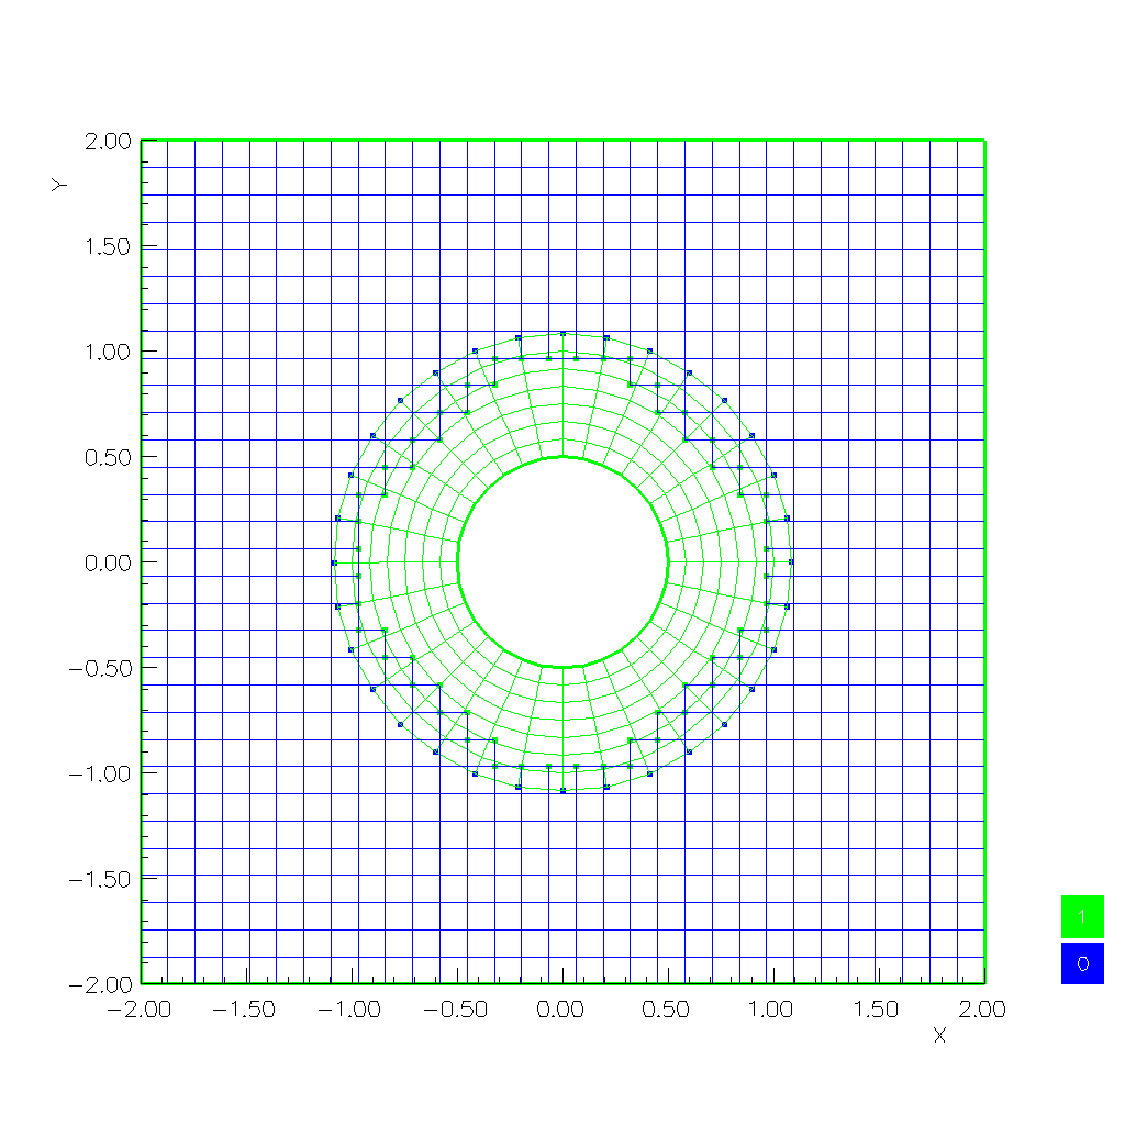
\includegraphics[width=\figWidthc]{\figures/cicDone}\\
  {Finished grid after removing excess interpolation points.}
  \end{center}


\vfill\eject
\subsection{Example: Valve}

These figures show the grid for a valve at various stages in the overlap algorithm.
\vglue-.1in
\begin{center}
 % 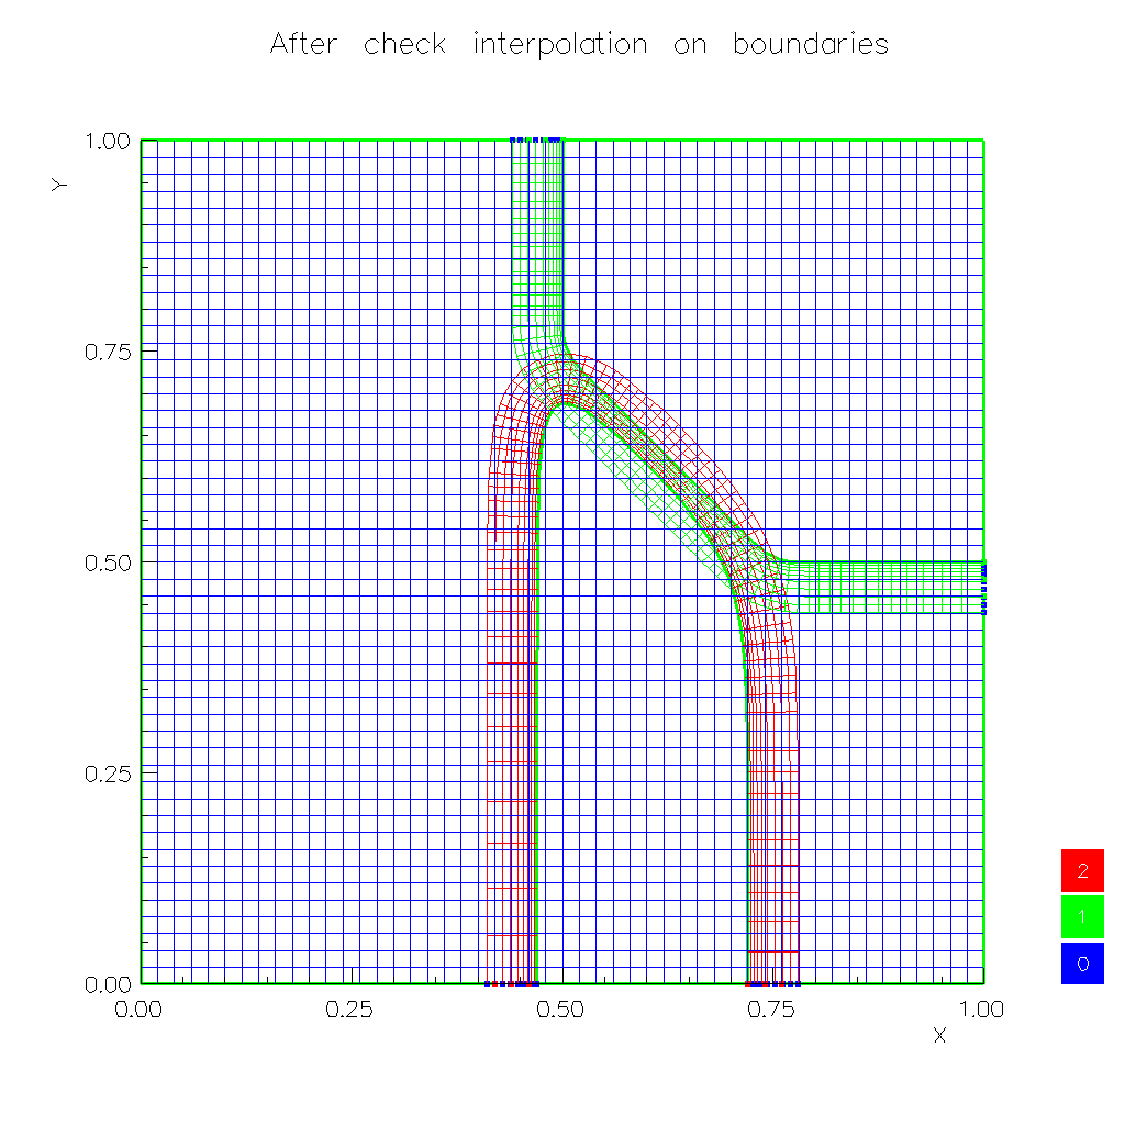
\epsfig{file=\figures/valveInterpBoundary.ps,height=\figHeight} \\
 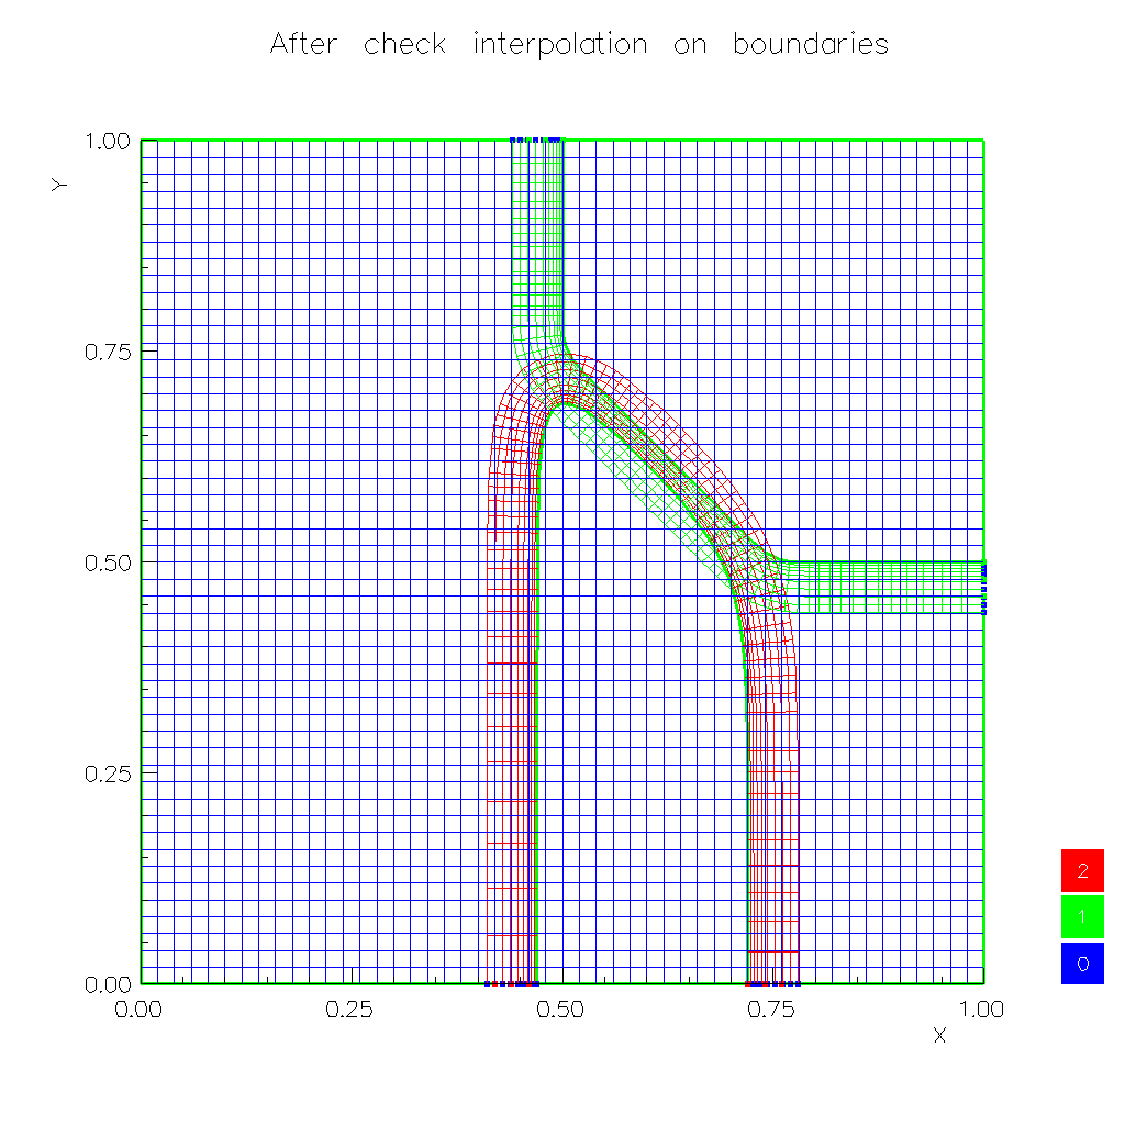
\includegraphics[width=\figWidthc]{\figures/valveInterpBoundary}\\
 {Grid after interpolation on boundaries.}
\end{center}
\vglue-.5in
\begin{center}
 % 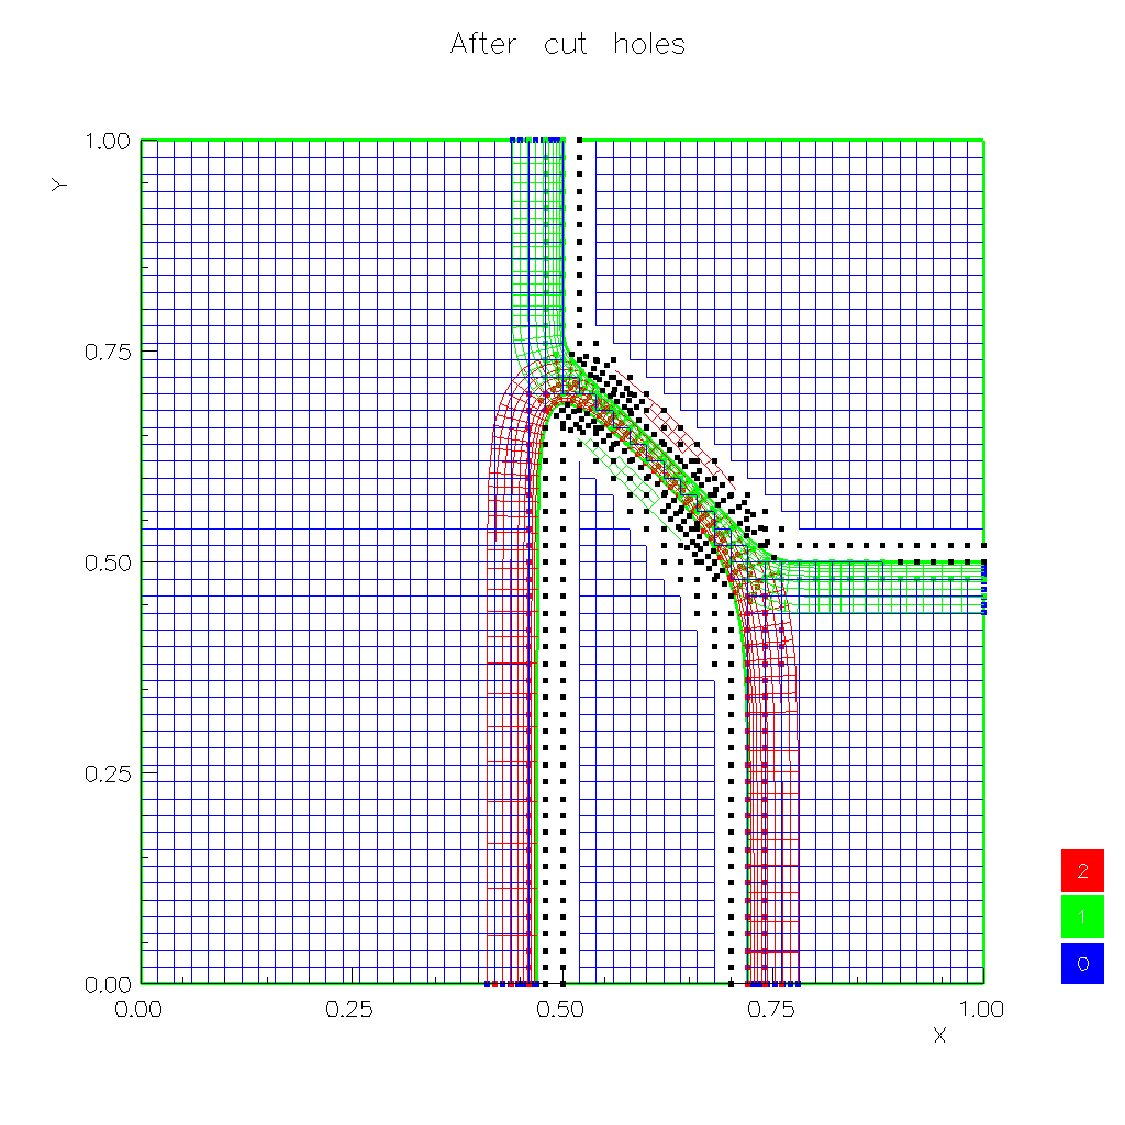
\epsfig{file=\figures/valveCutHoles.ps,height=\figHeight} \\
 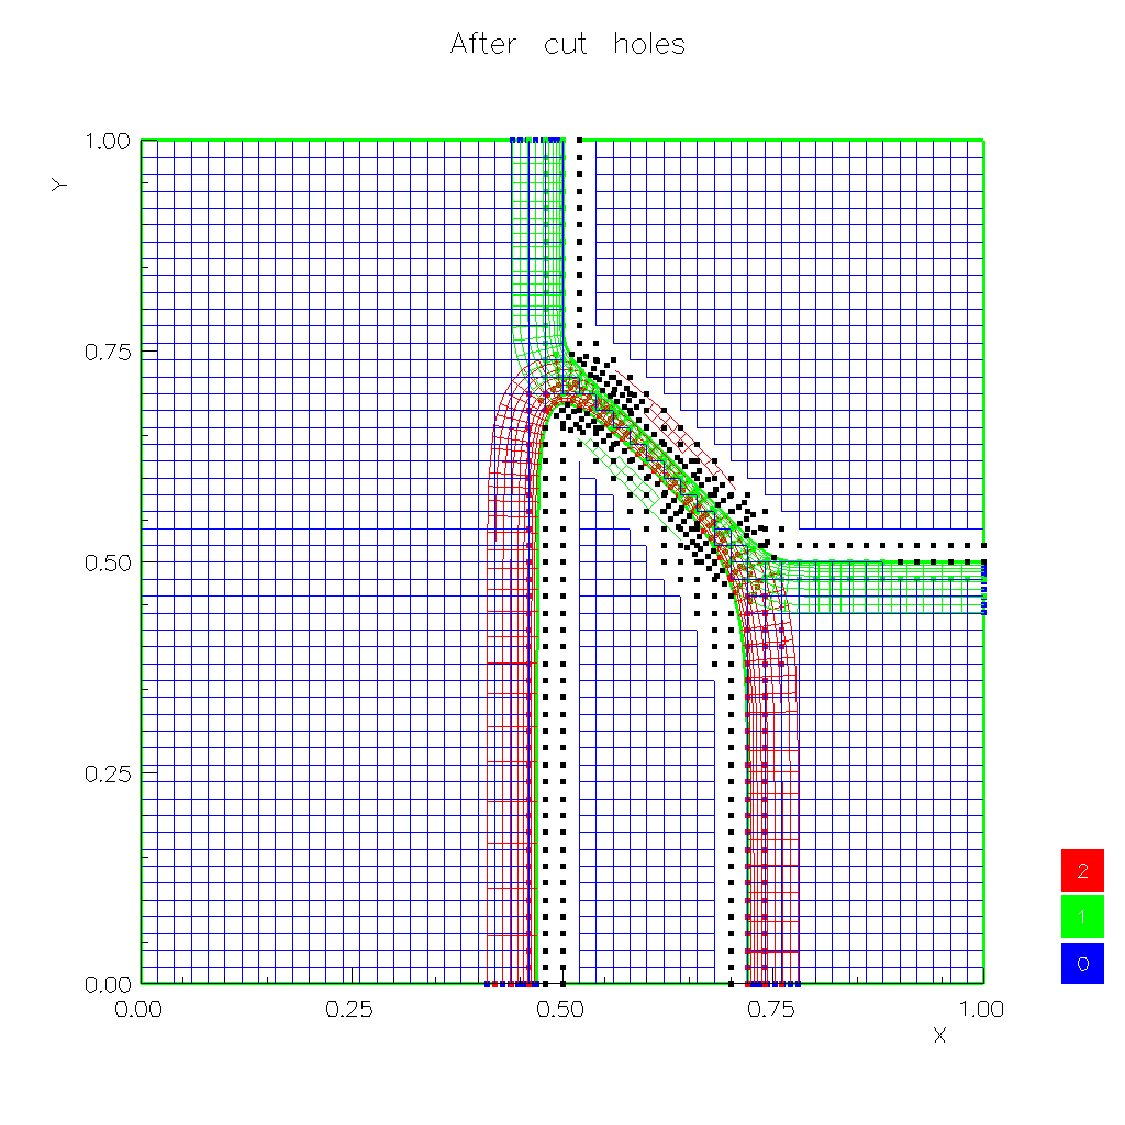
\includegraphics[width=\figWidthc]{\figures/valveCutHoles}\\
 {Grid after cutting holes. Physical boundaries are used to cut
      holes in nearby grids. The hole cutting algorithm will generate a barrier of hole points and
      interpolation points that bounds the entire hole region.}
\end{center}
\begin{center}
   % 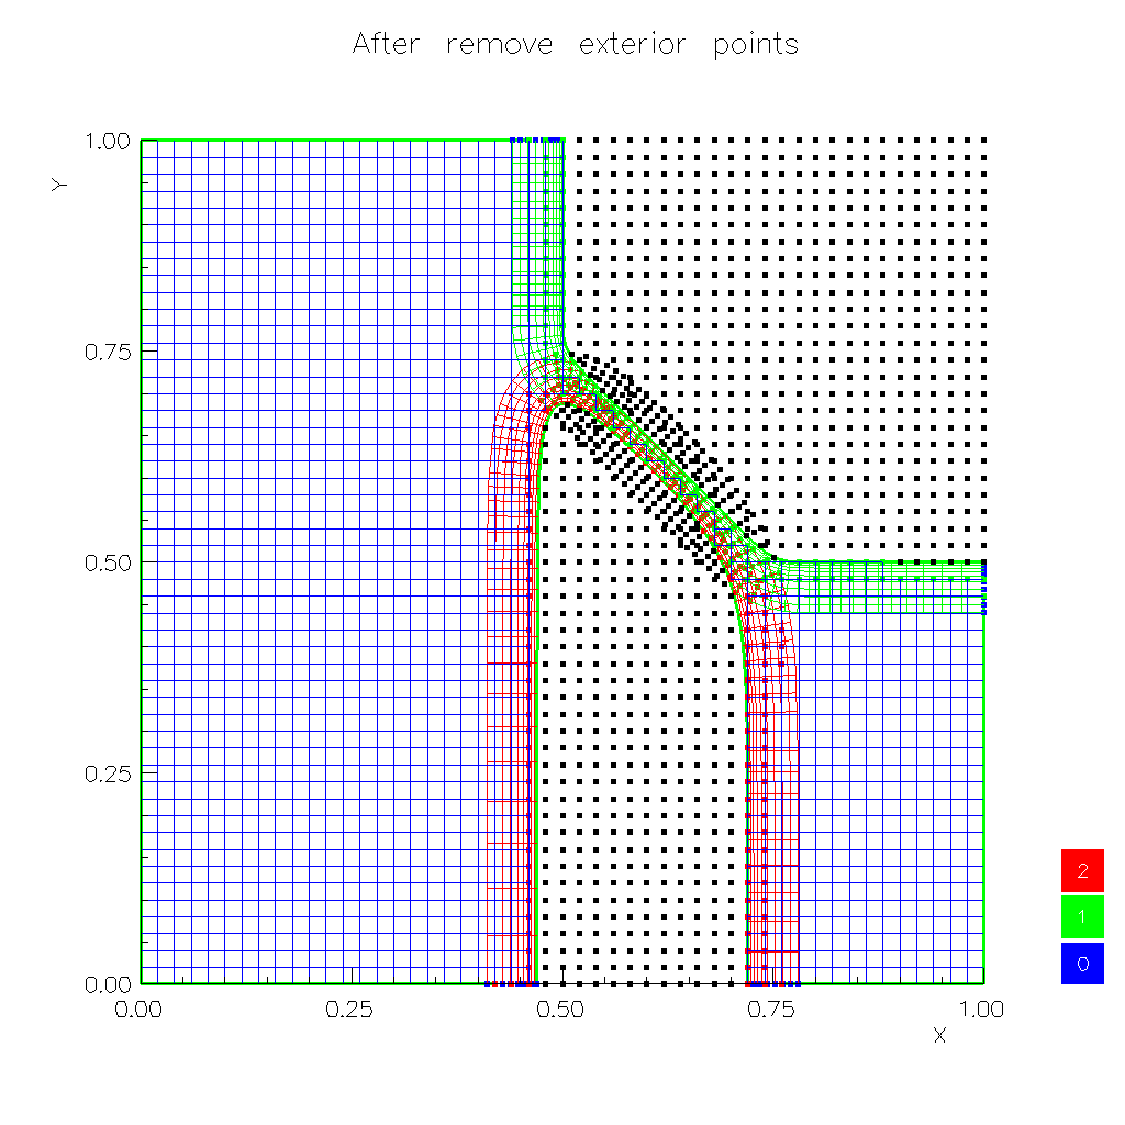
\epsfig{file=\figures/valveRemoveExterior.ps,height=\figHeight} \\
   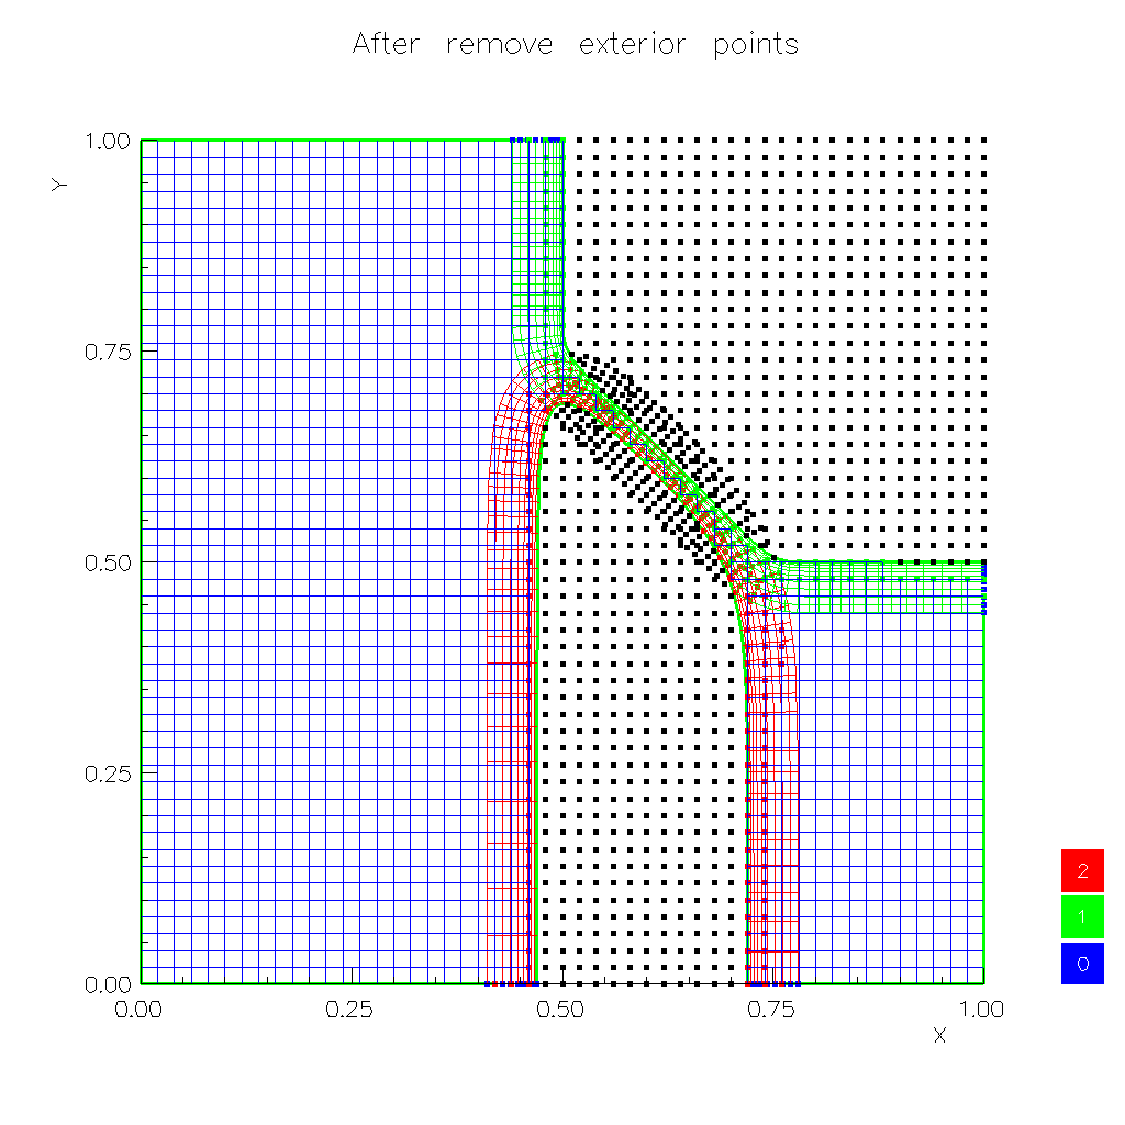
\includegraphics[width=\figWidthc]{\figures/valveRemoveExterior}\\
 {Grid after removing all exterior points. The exterior points are easily swept out
      after the hole boundary has been marked.}
  \end{center}
  \begin{center}
   % 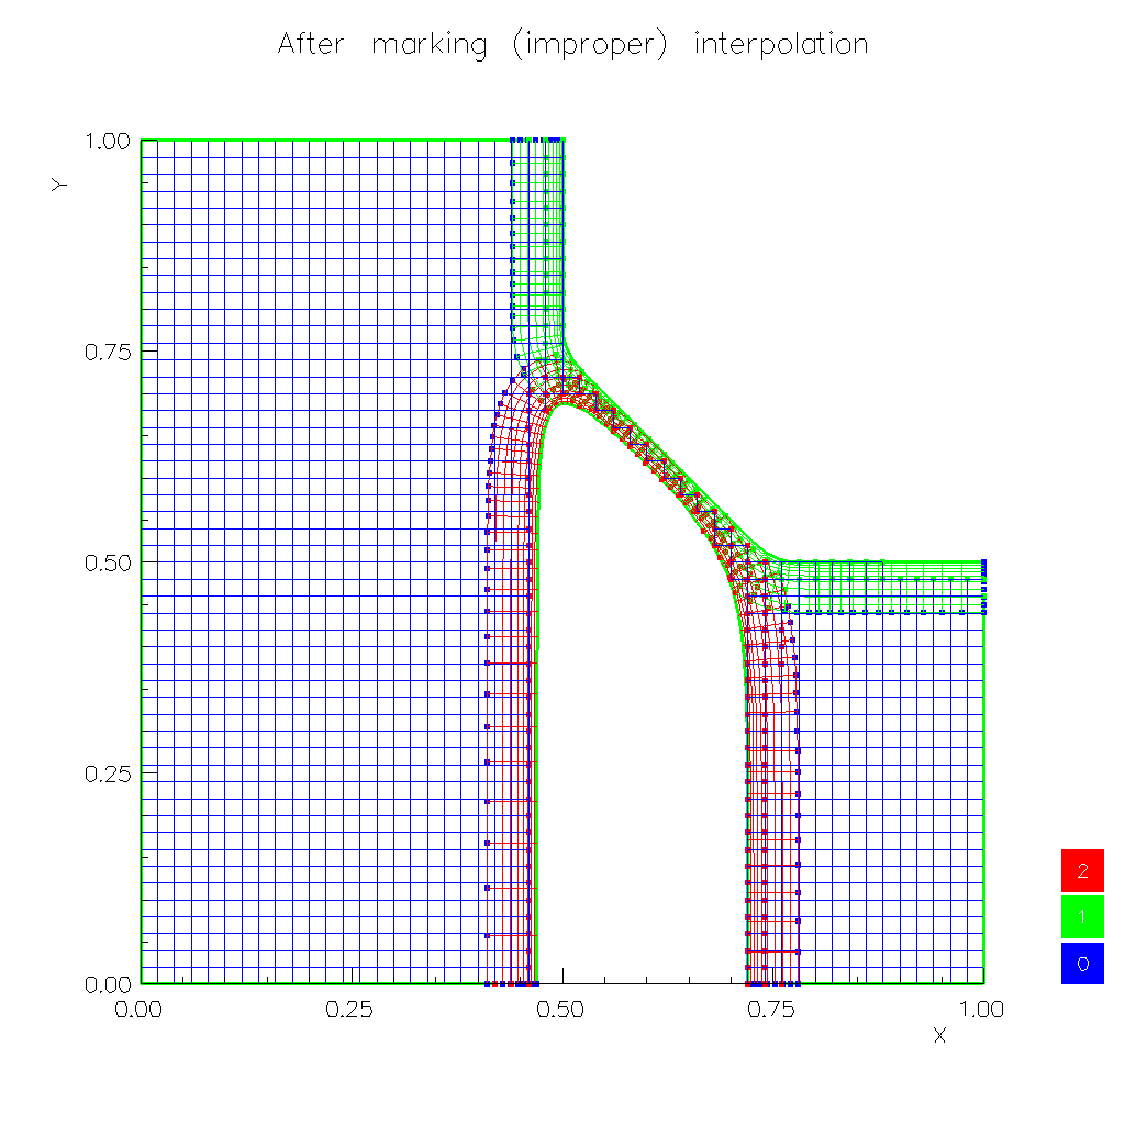
\epsfig{file=\figures/valveImproper.ps,height=\figHeight}  \\
   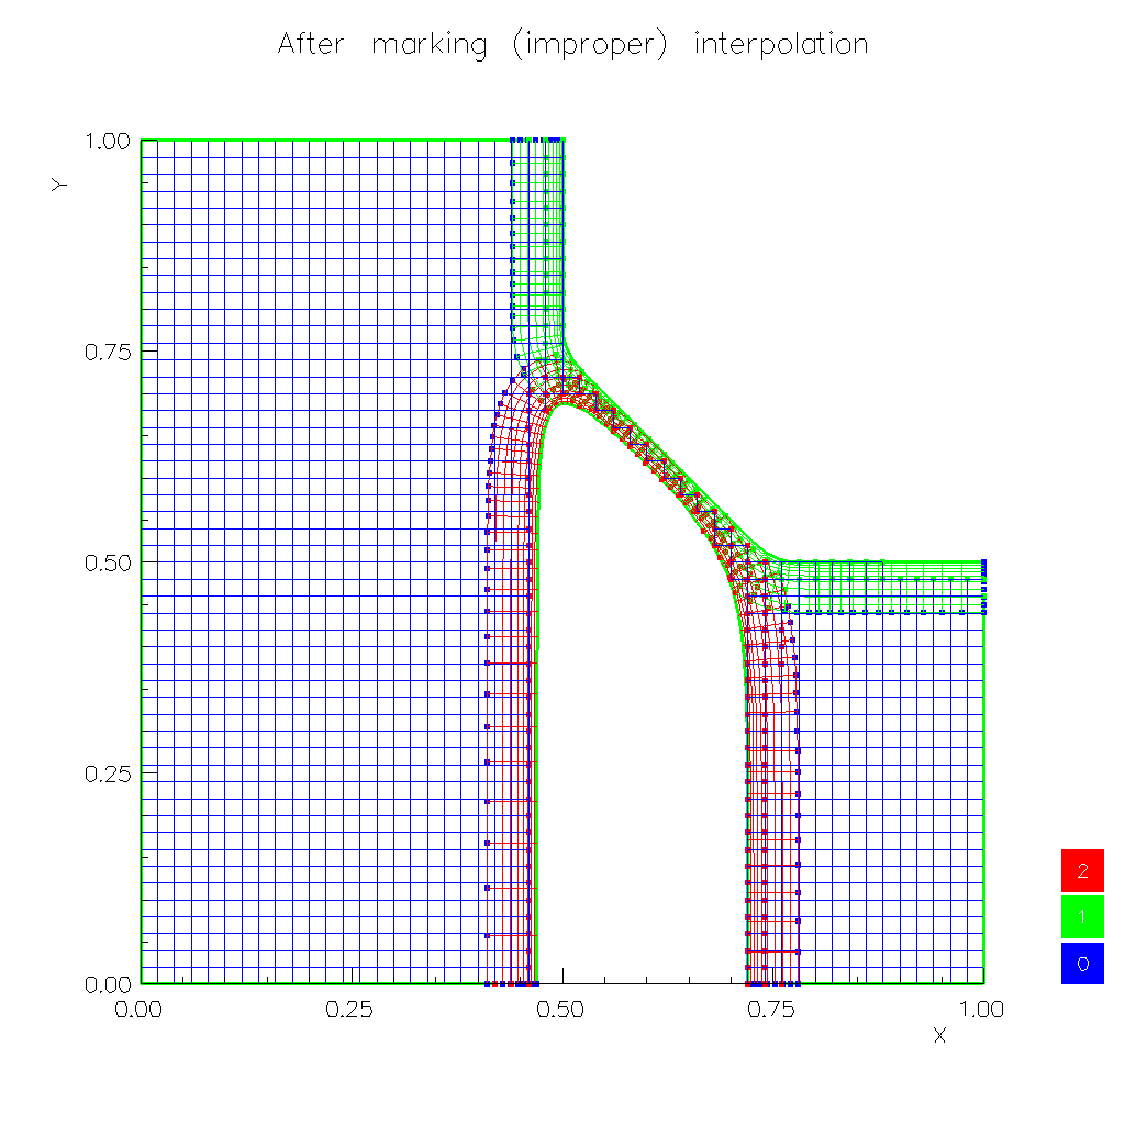
\includegraphics[width=\figWidthc]{\figures/valveImproper}\\
  {Grid after marking (improper) interpolation. These improper interpolation points need only lie
    inside another grid.}
  \end{center}
  \begin{center}
   % 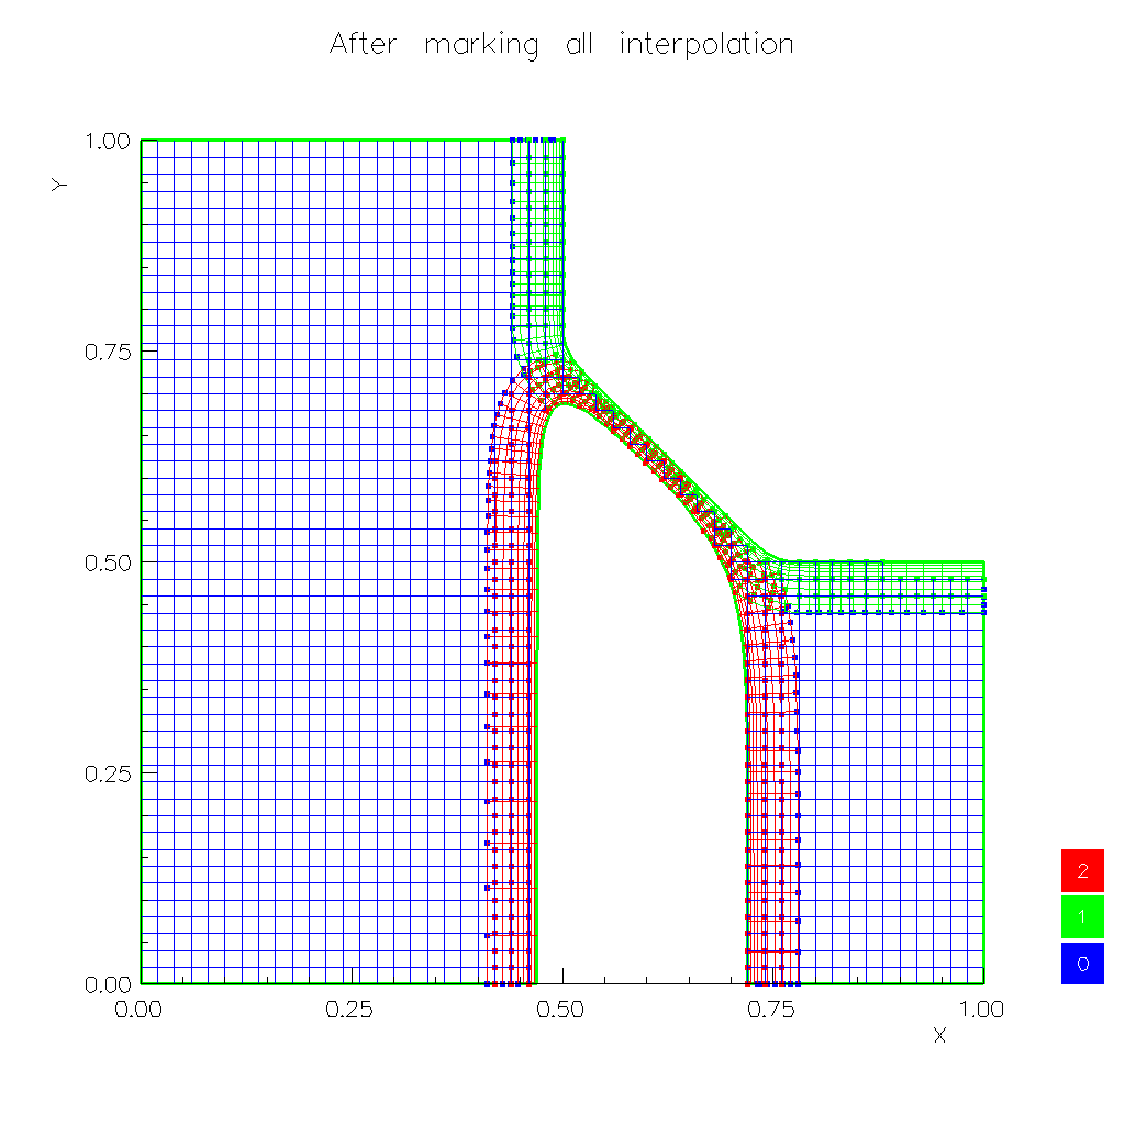
\epsfig{file=\figures/valveAll.ps,height=\figHeight} \\
   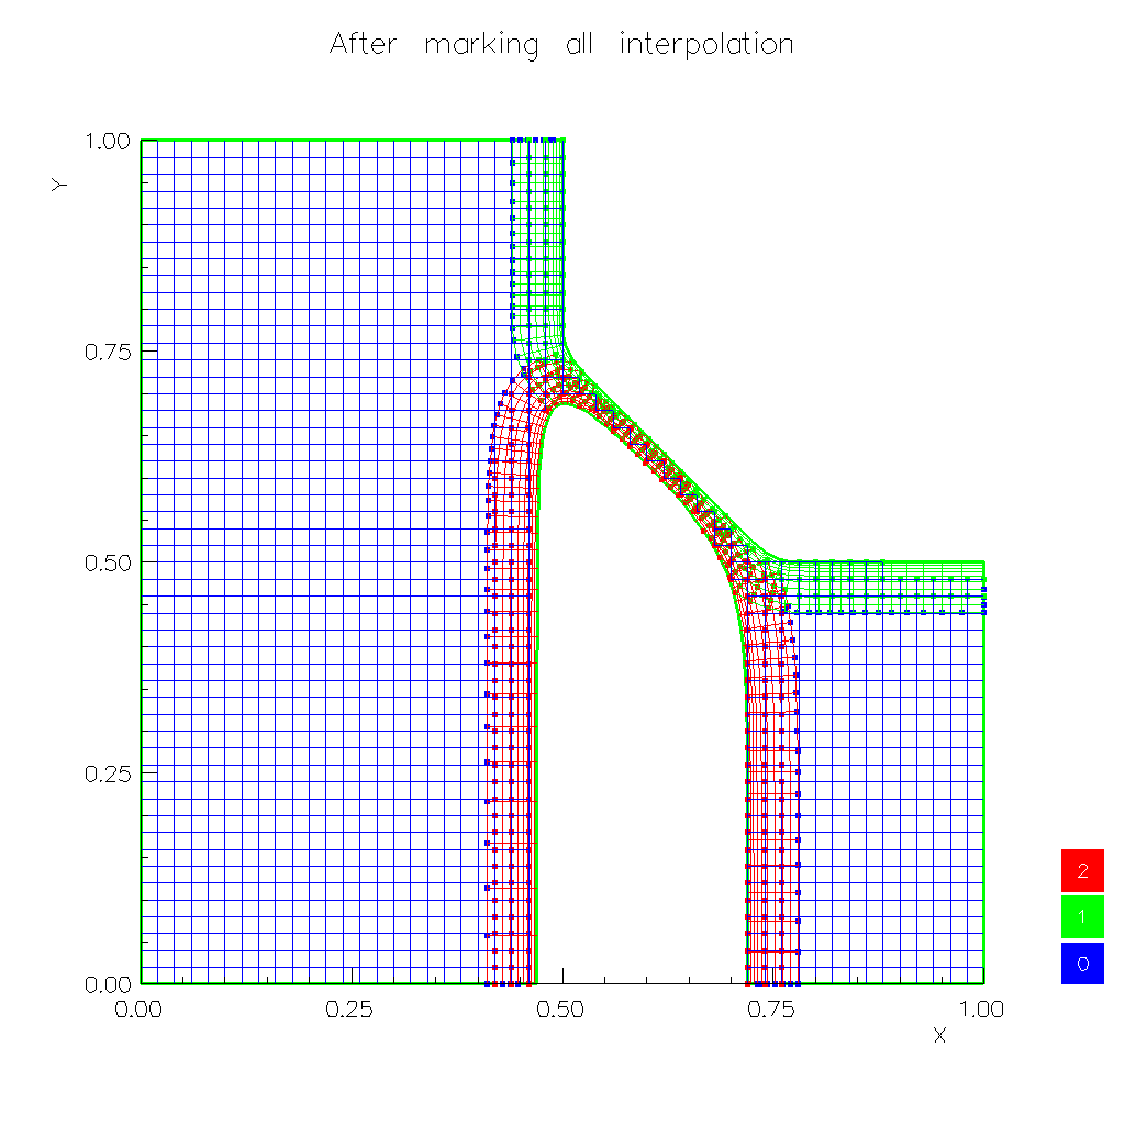
\includegraphics[width=\figWidthc]{\figures/valveAll}\\
  {Grid after marking all (proper) interpolation.}
  \end{center}
  \begin{center}
   % 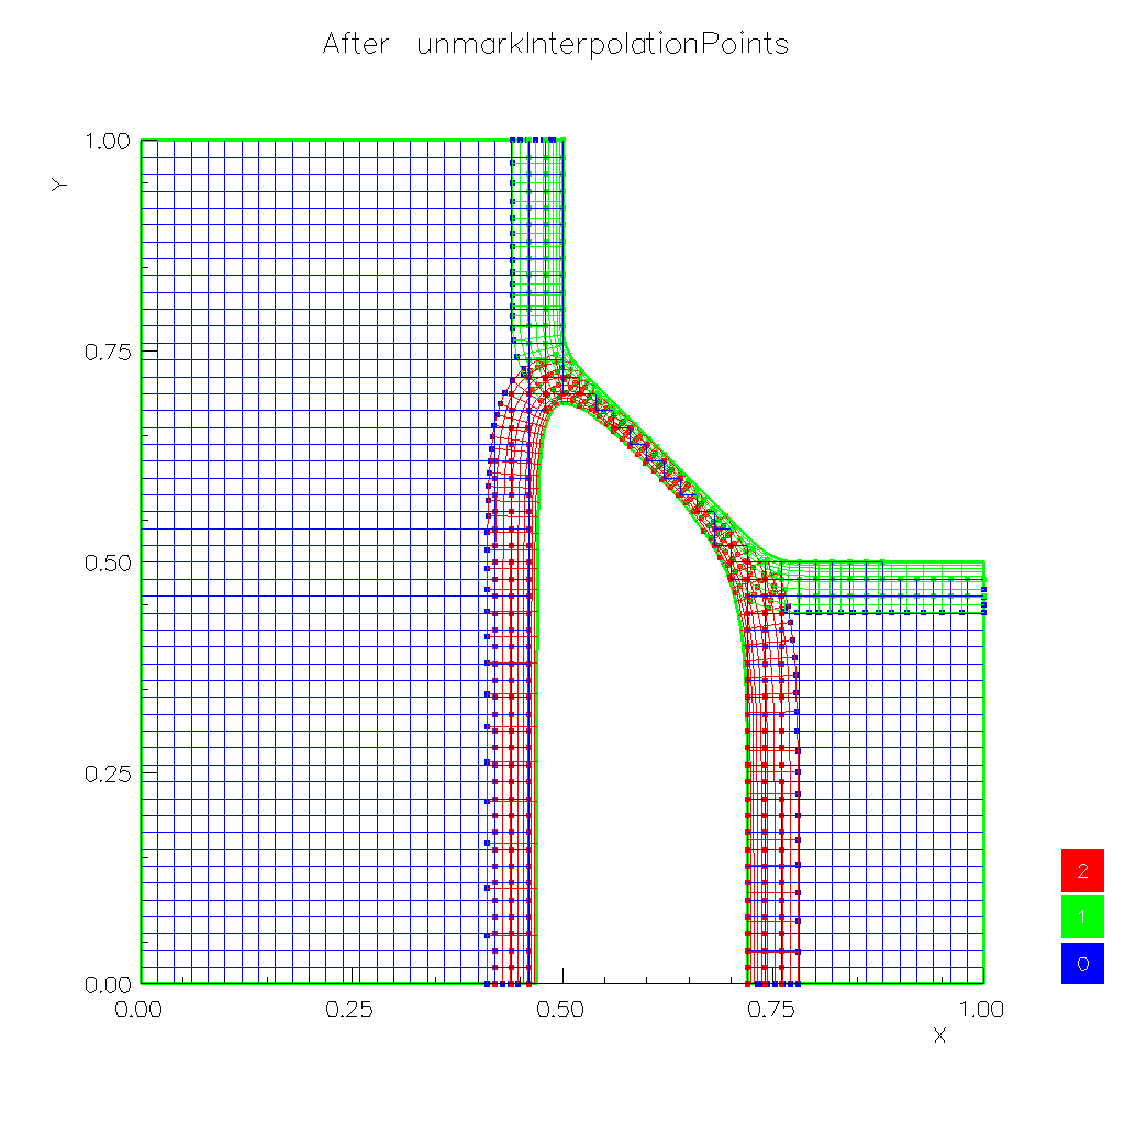
\epsfig{file=\figures/valveDone.ps,height=\figHeight} \\
   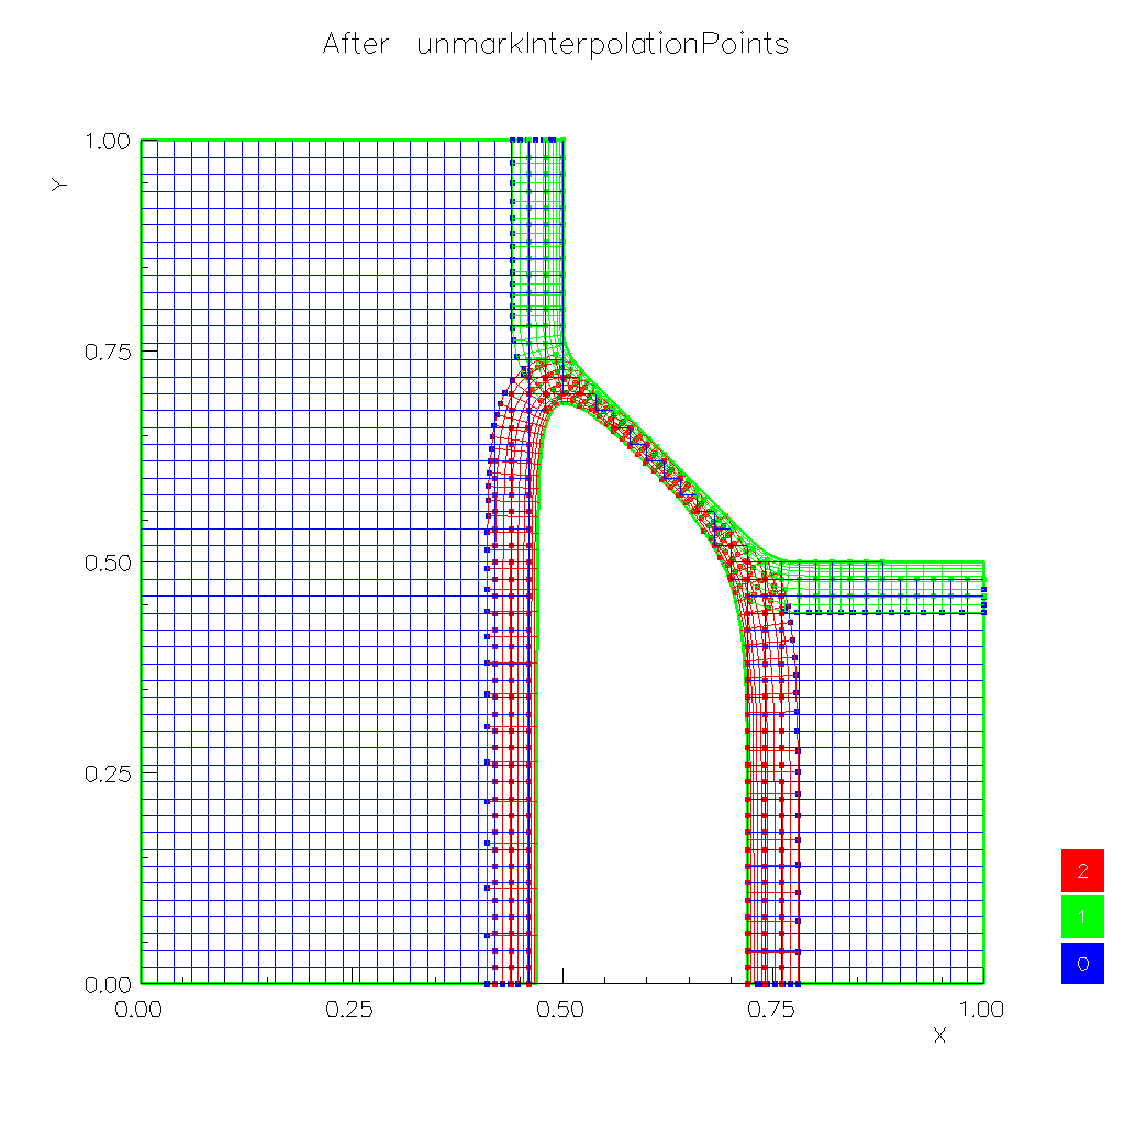
\includegraphics[width=\figWidthc]{\figures/valveDone}\\
  {Finished grid after removing excess interpolation points.}
  \end{center}


